% Перестроение расчетной сетки в двумерном случае.
\newpage
\section*{Глава 1. Перестроение поверхностной расчетной сетки в двумерном случае} % выключить номер первой главы
\addcontentsline{toc}{section}{Глава 1. Перестроение поверхностной расчетной сетки в двумерном случае} % но добавить ее в оглавление
\addtocounter{section}{1}                                                                             % а теперь и счетчик продвинуть
\setcounter{subsection}{0}
\setcounter{figure}{0}
\setcounter{equation}{0}
\setcounter{table}{0}
\setcounter{theorem}{0}
\setcounter{lemma}{0}
\setcounter{definition}{0}

В этой главе исследуется перестроение поверхностной расчетной сетки в двумерном случае применительно к моделированию обледенения.
Рассматриваются известные методы перестроения, предлагается новый метод и выводятся аналитические оценки точности и сглаживания дефектов на модельных сетках.
Перестроение расчетной сетки должно выполняться таким образом, чтобы заметаемая площадь плоскости при движении сетки соответствовала объему накопленного на поверхности льда.

Приведем кратко некоторые определения и соглашения касательно геометрических примитивов, которые будут использоваться в этой и последующих главах.

При рассмотрении геометрических объектов наряду с понятием точки $P = (P_x, P_y) = (x_P, y_P)$ в двумерном случае и $P = (P_x, P_y, P_z) = (x_P, y_P, z_P)$ в трехмерном случае будем использовать также понятие радиус-вектора $\overline{P}$, компонентами которого являются координаты этой точки.
В дальнейшем будем считать эти термины взаимозаменяемыми.

Прямую, проходящую через точку $A$ и направленную вдоль вектора $\overline{D}$, обозначаемую $Line(A, \overline{D})$, будем определять как геометрическое место точек (ГМТ\label{abbr:gmt-1}) $\overline{P}(\alpha)$ на плоскости или в пространстве, заданное следующим образом:
\begin{equation}\label{eqn:text_1_geo_prim_line}
	\overline{P}(\alpha) = \overline{A} + \alpha \overline{D}, \ \alpha \in \mathbb{R}
\end{equation}

Если даны две точки $A$ и $B$, то через $\overline{AB}$ будем обозначать вектор, направленный из точки $A$ в точку $B$ ($\overline{AB} = \overline{B} - \overline{A}$).

Отрезок с концами $A$ и $B$, обозначаемый $Segm(A, B)$, определяется как ГМТ $\overline{P}(\alpha)$ на плоскости или в пространстве, заданное следующим образом:

\begin{equation}\label{eqn:text_1_geo_prim_segment}
	\left\{
		\begin{aligned}
			& \overline{P}(\alpha) = \overline{A} + \alpha \overline{AB}, \ \alpha \in \mathbb{R} \\
			& 0 \le \alpha \le 1
		\end{aligned}
	\right.
\end{equation}

\begin{definition}
Двумерной поверхностной расчетной сеткой будем называть ломаную без самопересечений, состоящую из $n$ ячеек-отрезков $F_i$ длиной $l_i$ ($0 \le i < N$).
Ячейка $F_i$ имеет инцидентные узлы $N_i$, $N_{i + 1}$ ($F_i = Segm(N_i, N_{i + 1})$) и внешнюю единичную нормаль $\overline{n}_i^F$.
Если узлы с номерами $0$ и $n$ совпадают, то сетка является замкнутой.
Для узла $N_i$ определена единичная нормаль $\overline{n}_i^N = \frac{\overline{n}_{i-1}^F + \overline{n}_i^F)}{|\overline{n}_{i-1}^F + \overline{n}_i^F|}$, лежащая на биссектрисе телесного угла между ячейками $F_{i - 1}$ и $F_i$, обозначаемого $2 \phi_i$ (рис.~\ref{fig:text_1_remesh_2d_grid_normals}).
\end{definition}

\begin{figure}[ht]
\centering
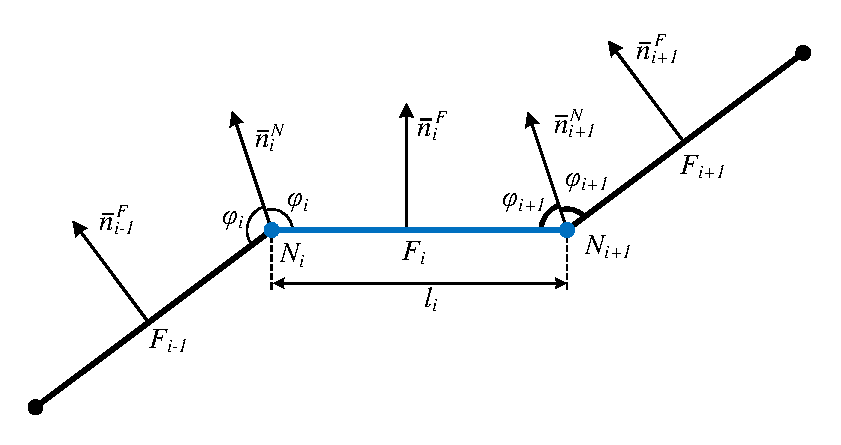
\includegraphics[width=0.7\textwidth]{fig/2dr_grid_normals.pdf}
\singlespacing
\captionstyle{center}\caption{Поверхностная расчетная сетка с обозначенными \\ нормалями ячеек и узлов.}
\label{fig:text_1_remesh_2d_grid_normals}
\end{figure}

Пусть известно, что за некий малый промежуток времени $i$-ая ячейка сдвигается в направлении своей нормали на некоторую величину $H_i$, где $H_i$ -- вычисленная высота ледяного покрова в ячейке $F_i$

\begin{definition}
Целевой площадью для $i$-ой ячейки будем называть величину $T_i = l_i H_i$ -- площадь, заметаемая $i$-ой ячейкой при смещении на величину $H_i$ в направлении своей внешней нормали.
\end{definition}

Если просто сдвинуть каждую ячейку в направлении своей нормали, то сетка потеряет целостность, поэтому мы можем осуществлять движение только узлов.
Для моделирования процесса ледообразования центральной задачей перестроения поверхностной сетки является определение новых положений узлов $N'_i$, при которых площадь $S_i = S_{N_iN'_iN'_{i+1}N_{i+1}}$, заметаемая ячейкой $F_i$, как можно меньше отличается от целевой площади $T_i$.
Задача рассматривается при фиксированных направлениях смещения узлов вдоль их нормалей $\overline{n}_i^N$ \cite{Fortin2004Remesh2d}, то есть требуется определить только величины смещения узлов $h_i$.
Для оценки отклонения заметаемой площади от целевой используются обозначения: $\Delta_i = S_i - T_i$ -- абсолютное отклонение от целевой площади, $\delta_i = \frac{\Delta_i}{T_i}$ -- относительное отклонение от целевой площади.
Новая перестроенная поверхностная сетка соответствует поверхности ледяного покрова, а общая заметаемая площадь при движении поверхности соответствует объему накопленного на поверъности льда.

%---------------------------------------------------------------------------------------------------

\subsection{Определение смещений узлов в общем случае}

Рассмотрим геометрическую задачу о перестроении поверхности в двумерном случае в общем виде \cite{Rybakov2019Geo2D}.
Для решения поставленной задачи сначала требуется вычислить заметаемую площадь для каждой отдельной ячейки.
Затем, просуммировав заметаемые площади для всех ячеек, можно получить площадь, заметаемую при движении сетки целиком.

\subsubsection{Задача о вычислении заметаемой площади при движении узлов отдельной ячейки}

Рассматривается ячейка, представленная на плоскости отрезком $AB$ длины $l$.
При перемещении точек $A$ и $B$ в новые точки $A'$ и $B'$ соответственно образуется четырехугольник $AA'B'B$.
Требуется найти его площадь, выраженную явно через параметры $a = AA'$ и $b = BB'$ и углы при вершинах $A$ и $B$ (рис.~\ref{fig:text_1_remesh_2d_local}).

\begin{figure}[ht]
\centering
\begin{tabular}{ll}
	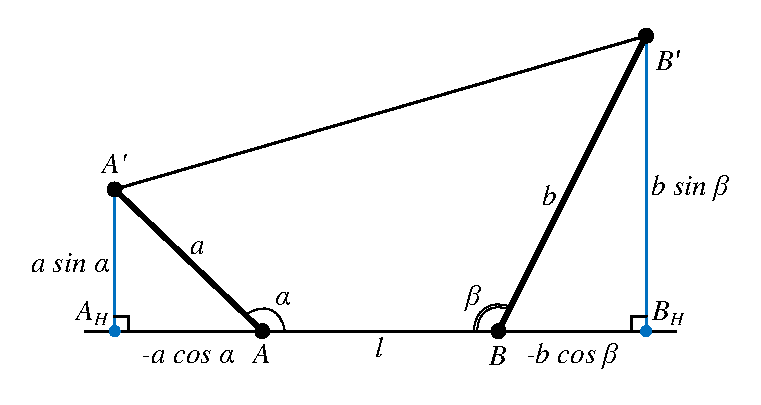
\includegraphics[width=0.45\textwidth]{fig/2dr_remesh_local.pdf}
	&
	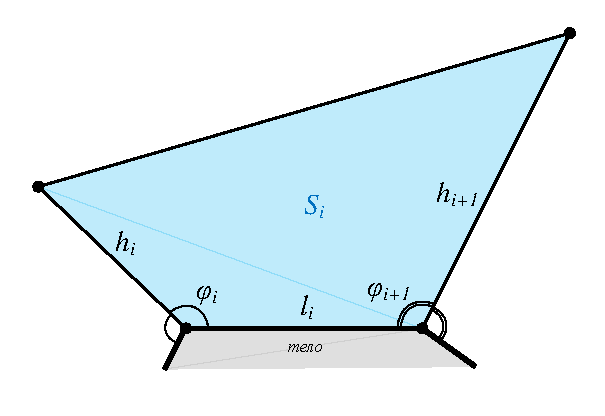
\includegraphics[width=0.38\textwidth]{fig/2dr_remesh_local2.pdf}
\end{tabular}
\singlespacing
\captionstyle{center}\caption{Вычисление заметаемой площади через смещения узлов ячейки.}
\label{fig:text_1_remesh_2d_local}
\end{figure}

\begin{lemma}\label{lem:text_1_remesh_2d_AA1B1B}
Пусть дан четырехугольник $AA'B'B$, в котором $AA' = a$, $BB' = b$, $\angle A'AB = \alpha$, $\angle B'BA = \beta$.
Тогда площадь этого четырехугольника выражается формулой
\begin{equation}\label{eqn:text_1_remesh_2d_one_cell_lemma}
S_{AA'B'B} = \frac{1}{2} \left( l (a \sin \alpha + b \sin \beta) - ab \sin (\alpha + \beta) \right)
\end{equation}
\end{lemma}

Опустим перпендикуляры из точек $A'$ и $B'$ на прямую $AB$.
Их основаниями будут точки $A_H$ и $B_H$ соответственно.
Если $\alpha \ge \frac{\pi}{2}$, то перпендикуляр $A'A_H$ проходит снаружи четырехугольника $AA'B'B$, в противном случае -- внутри.
Аналогично, если $\beta \ge \frac{\pi}{2}$, то перпендикуляр $B'B_H$ проходит снаружи четырехугольника $AA'B'B$, в противном случае -- внутри.
В любом случае искомая площадь может быть представлена в следующем виде:
\begin{equation}
S_{AA'B'B} = S_{A_HA'B'B_H} - \sign \left( \alpha - \frac{\pi}{2} \right) S_{AA'A_H} - \sign \left( \beta - \frac{\pi}{2} \right) S_{BB'B_H}
\end{equation}

Эту площадь можно выразить явно через значения углов $\alpha$ и $\beta$:
\begin{multline}\label{eqn:2dr_local_square_abalphabeta}
S_{AA'B'B} = \frac{1}{2}(l - a \cos \alpha - b \cos \beta)(a \sin \alpha + b \sin \beta) \\ + \frac{1}{2}a^2 \sin \alpha \cos \alpha + \frac{1}{2}b^2 \sin \beta \cos \beta
\end{multline}

После раскрытия скобок и преобразований получим \eqref{eqn:text_1_remesh_2d_one_cell_lemma}.
$\blacksquare$\\

Отметим, что если $\alpha + \beta \ge \pi$ то $S_{AA'B'B}$ всегда положительна и возрастает с ростом $a$ или $b$.
Это означает, что лучи $AA'$ и $BB'$ не пересекаются (этот случай изображен на рис.~\ref{fig:text_1_remesh_2d_local}).

Рассмотрим случай $\alpha + \beta < \pi$.
Запишем отдельно условия неубывания $S_{AA'B'B}$ при росте $a$ и $b$:
\begin{equation}
	\begin{aligned}
		& \frac{\partial S_{AA'B'B}}{\partial a} = \frac{1}{2}(l \sin \alpha - b \sin (\alpha + \beta)) \ge 0 \\
		& \frac{\partial S_{AA'B'B}}{\partial b} = \frac{1}{2}(l \sin \beta - a \sin (\alpha + \beta)) \ge 0
	\end{aligned}
\end{equation}
или
\begin{equation}\label{eqn:text_1_remesh_2d_cond_abl}
	\begin{aligned}
		& a \le \frac{l \sin \beta}{\sin (\alpha + \beta)} \\
		& b \le \frac{l \sin \alpha}{\sin (\alpha + \beta)}
	\end{aligned}
\end{equation}

Если выполняются оба условия из \eqref{eqn:text_1_remesh_2d_cond_abl}, то четырехугольник $AA'B'B$ продолжает оставаться выпуклым.
Если выполнятеся только одно условие из \eqref{eqn:text_1_remesh_2d_cond_abl}, то четырех угольник является невыпуклым.
Если не выполняется ни одно из условий \eqref{eqn:text_1_remesh_2d_cond_abl}, то произошло самопересечение сетки, то есть оба отрезка $AA'$ и $BB'$ вышли за пределы треугольника $ABO$, где $O$ -- точка пересечения лучей $AA'$ и $BB'$.
Случаи самопересечения должны быть обработаны отдельно для возможности продолжения работы с расчетной сеткой.
В этой главе вопросы самопересечения расчетной сетки не рассматриваются, они будут рассмотрены в третьей главе в общей трехмерной постановке.

\subsubsection{Поиск смещений узлов методом градиентного спуска}

Метод градиентного спуска является одним из наиболее простых методов оптимизации для нахождения локального минимума функции ($f(x)$).
При условии, что в любой точке функции можно вычислить ее градиент, то начиная с некоторого начального приближения $x_0$, находящегося в окрестности локального минимума, строится итерационная последовательность~\cite{Kantorovich1984Func}:
\begin{equation}
x_{k+1} = x_k - \gamma_k \nabla f(x_k)
\end{equation}
где $\gamma_k \ge 0$ задает длину шага и, соответственно, скорость градиентного спуска.

Метод градиентного спуска находит свое основное применение в задаче поиска минимума или максимума функции.
Направление антиградиента является направлением наискорейшего убывания функции.
Основная проблема метода заключается в выборе шага $\gamma$.
При слишком больших значениях шага существует вероятность миновать искомый минимум функции.
К тому же, метод не гарантирует нахождение глобальных экстремумов.

Рассмотрим решение задачи определения величин смещения узлов поверхностной расчетной сетки при перестроении методом градиентного спуска.
Неизвестными параметрами являются величины сдвигов узлов сетки $h_i$ для $0 \le i \le n$.
Опираясь на решение локальной задачи об определении заметаемой площади из леммы~\ref{lem:text_1_remesh_2d_AA1B1B}, можно записать заметаемую площадь при движении отдельной ячейки (см. рис.~\ref{fig:text_1_remesh_2d_local} справа):
\begin{equation}
S_i = \frac{1}{2} \left( l_i(h_i \sin \phi_i + h_{i + 1} \sin \phi_{i+1}) - h_ih_{i + 1} \sin(\phi_i + \phi_{i+1}) \right)
\end{equation}

Для нахождения решения задачи перестроения поверхностной сетки в соответствии с методом наименьших квадратов будем искать минимум функции
\begin{equation}
D(\overline{h}) = D(h_0, \dots, h_{n}) = \sum_{i = 0}^{n - 1}{\Delta_i^2}
\end{equation}

Для нахождения градиента требуется вычислить частные производные $\frac{\partial D}{\partial h_i}$.
Эти частные производные можно записать в явном виде:
\begin{equation}
\frac{\partial D}{\partial h_i} = \frac{\partial (\Delta_{i - 1})^2}{\partial h_i} + \frac{\partial (\Delta_i)^2}{\partial h_i}
\end{equation}
где
\begin{equation}
\begin{cases}
\frac{\partial (\Delta_{i - 1})^2}{\partial h_i} = \Delta_{i - 1} (l_{i - 1} \sin \phi_i - h_{i - 1} \sin(\phi_{i - 1} + \phi_i)) \\
\frac{\partial (\Delta_i)^2}{\partial h_i} = \Delta_i (l_i \sin \phi_i - h_{i + 1} \sin(\phi_i + \phi_{i+1}))
\end{cases}
\end{equation}

\

Также при осуществлении метода градиентного спуска требуется следить за соблюдением дополнительных условий, которые накладываются на неизвестные $h_i$.
Например, очевидным условием является выполнение соотношения $h_i \ge 0$, что запрещает движение узлов сетки в отрицательном направлении.
Также можно использовать более строгие условия $\min(H_{i - 1}, H_i) \le h_i \le \max(H_{i - 1}, H_i)$, которые не позволят величинам смещения узлов сетки выходить за пределы смещений инцидентных им ячеек сетки.

Решение задачи о перестроении сетки методом градиентного спуска оказывается слишком требовательным к вычислительным ресурсам при увеличении размера сетки.
К тому же качество решения зачастую оказывается неудовлетворительным при попадании в локальные минимумы.
Поэтому рассматриваются приближенные методы перестроения.

%---------------------------------------------------------------------------------------------------

\subsection{Приближенные методы перестроения}

Для решения задачи перестроения расчетной сетки в двумерном случае рассмотрим приближенные методы, основанные на представлении целевой площади в виде примитивных геометрических фигур.

\begin{figure}[ht]
\centering
\begin{tabular}{ll}
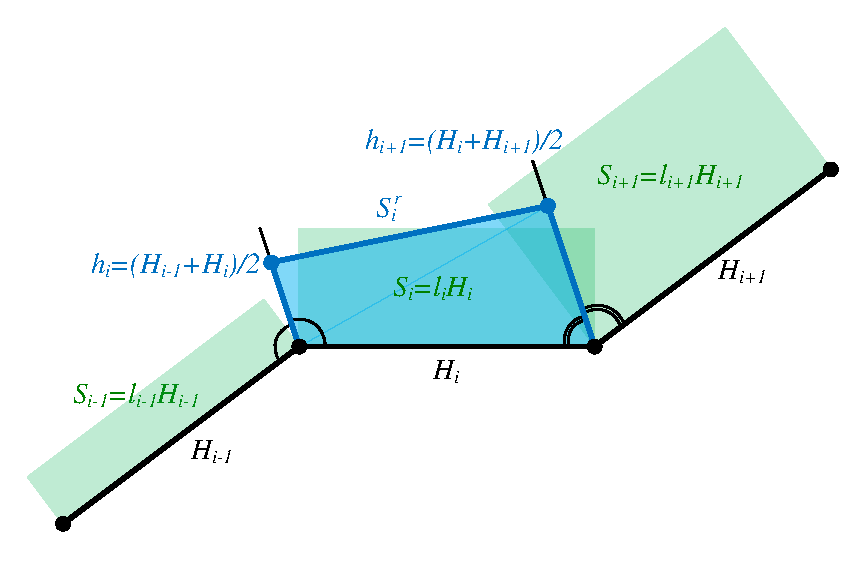
\includegraphics[width=0.45\textwidth]{fig/2dr_remesh_rectangles.pdf}
&
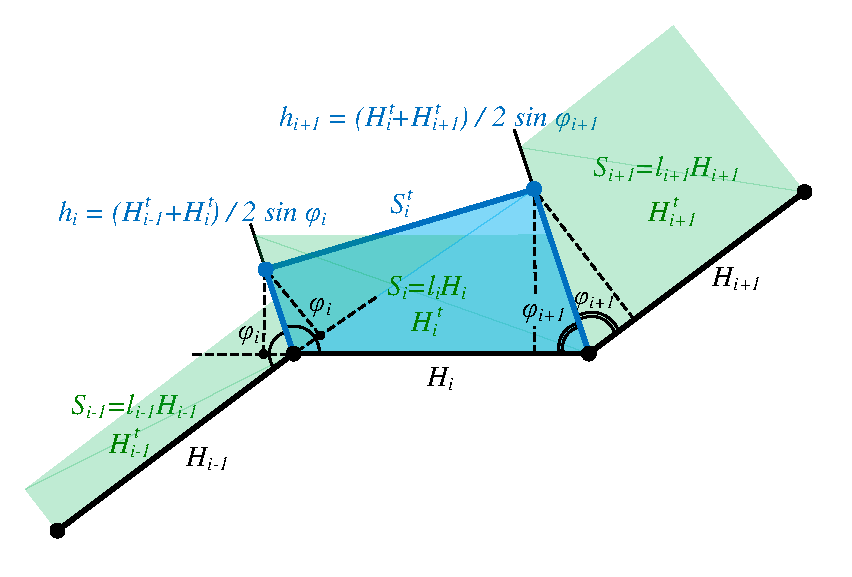
\includegraphics[width=0.45\textwidth]{fig/2dr_remesh_trapeziums.pdf}
\end{tabular}
\singlespacing
\captionstyle{center}\caption{Перестроение поверхностной расчетной сетки методом прямоугольников (слева) и трапеций (справа).}
\label{fig:text_1_remesh_2d_rectangles_and_trapeziums}
\end{figure}

\subsubsection{Метод прямоугольников}

В качестве первого метода перестроения поверхностной расчетной сетки рассмотрим приближение, при котором целевая площадь для $i$-ой ячейки представлена прямоугольником со сторонами $l_i$ и $H_i$.
В качестве величины смещения узла берется среднее арифметичское двух высот инцидентных ячеек $h_i = \frac{H_{i - 1} + H_i}{2}$ (см. рис.~\ref{fig:text_1_remesh_2d_rectangles_and_trapeziums} слева).
Этот метод перестроения будем называть методом прямогольников.
Заметаемую $i$-ой ячейкой площадь при использовании метода прямоугольников будем обозначать $S_i^r$, а также обозначим абсолютное и относительное отклонения от целевой площади через $\Delta_i^r = S_i^r - T_i$ и $\delta_i^r = \frac{\Delta_i^r}{T_i}$ соответственно.

\subsubsection{Заметаемая площадь при параллельном смещении ячейки}\label{sec:text_1_geo_prim_volume}

Для рассмотрения второго метода перестроения расчетной сетки приведем решение следующей задаче.

Рассмотрим отрезок $Segm(A, B)$.
Пусть известно направление единичной нормали этого отрезка $\overline{n}$, а также направления движения его концов $\overline{n}_A$, $\overline{n}_B$.
Пусть на расстоянии $h$ от прямой $AB$ проходит параллельная прямая, пересекающая направления $\overline{n}_A$, $\overline{n}_B$ в точках $A'$ и $B'$ соответственно.
Требуется найти зависимость площади трапеции $S_{AA'B'B}$ от расстояния между прямыми $h$ (см. рис.~\ref{fig:text_1_geo_prim_trapezoid_partial}).

\begin{figure}[ht]
\centering
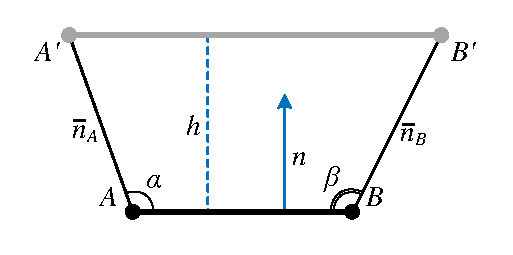
\includegraphics[width=0.45\textwidth]{fig/2dr_trapezoid_partial.pdf}
\singlespacing
\captionstyle{center}\caption{Заметаемая площадь при движении концов отрезка.}
\label{fig:text_1_geo_prim_trapezoid_partial}
\end{figure}

Рассмотрим движение точки $A$.
Пусть $\overline{A}' = \overline{A} + t \overline{n}_A$.
Так как расстояние между прямыми $AB$ и $A'B'$ равно $h$, то $(t \overline{n}_A, \overline{n}) = h$, откуда получаем $t = \frac{h}{(\overline{n}_A, \overline{n})}$.

Вычисляя положения точек $A'$ и $B'$, можно получить выражение для площади трапеции $AA'B'B$.
\begin{equation}\label{eqn:text_1_geo_prim_aa1b1b}
	\begin{aligned}
		& \overline{A}' = \overline{A} + h \overline{u}_A, \ \overline{u}_A = \frac{\overline{n}_A}{(\overline{n}_A, \overline{n})} \\
		& \overline{B}' = \overline{B} + h \overline{u}_B, \ \overline{u}_B = \frac{\overline{n}_B}{(\overline{n}_B, \overline{n})} \\
		& S_{AA'B'B}(h) = \frac{1}{2} \left( |\overline{A} - \overline{B}| + |\overline{A}' - \overline{B}'| \right) h
	\end{aligned}
\end{equation}

Отметим один частный случай, в котором трапеция $AA'B'B$ является равнобокой с углом $\alpha$ при основании $AB$.
Тогда при $AB = l$ имеем $A'B' = l - 2 h \ctg \alpha$, и
\begin{equation}
	S_{AA'B'B}(h) = (l - h \ctg \alpha) h
\end{equation}
откуда $h$ может быть выражена с помощью решения квадратного уравнения
\begin{equation}\label{eqn:text_1_geo_prim_trapezium_h_from_s}
	h(S, l, \alpha) = \frac{l - \sqrt{l^2 - 4 S \ctg \alpha}}{2 \ctg \alpha}
\end{equation}

\subsubsection{Метод трапеций}

В качестве второго метода перестроения поверхностной расчетной сетки будем рассматривать метод трапеций.
В методе трапеций целевая площадь $i$-ой ячейки представляется трапецией с площадью $T_i$.
Боковые стороны этой трапеции лежат на направлениях движения двух узлов, инцидентных рассматриваемой ячейке.
Высота трапеции $H_i^t$ находится из \eqref{eqn:text_1_geo_prim_aa1b1b} с помощью решения квадратного уравнения.
После построения трапеций для всех ячеек сетки у каждого узла появляется две новые потенциальные позиции для сдвига (образованные ячейкой слева и ячейкой справа).
В качестве финальной новой позиции выбирается их среднее значение (рис.~\ref{fig:text_1_remesh_2d_rectangles_and_trapeziums} справа).
Таким образом, величина смещения узла определяется как $h_i = \frac{H_{i - 1}^t + H_i^t}{2 \sin \phi_i}$.
Заметаемую $i$-ой ячейкой площадь при использовании метода трапеций будем обозначать $S_i^t$, а абсолютное и относительное отклонения от целевой площади -- $\Delta_i^t = S_i^t - T_i$ и $\delta_i^t = \frac{\Delta_i^t}{T_i}$ соответственно.

\subsubsection{Метод окрестностей в двумерном случае}\label{sec:2dr_okrestnost_method}

Предлагается новый метод перестроения поверхностной расчетной сетки, который будем называть методом окрестностей (см. рис.~\ref{fig:text_1_remesh_2d_okrestnost}).

\begin{figure}[ht]
\centering
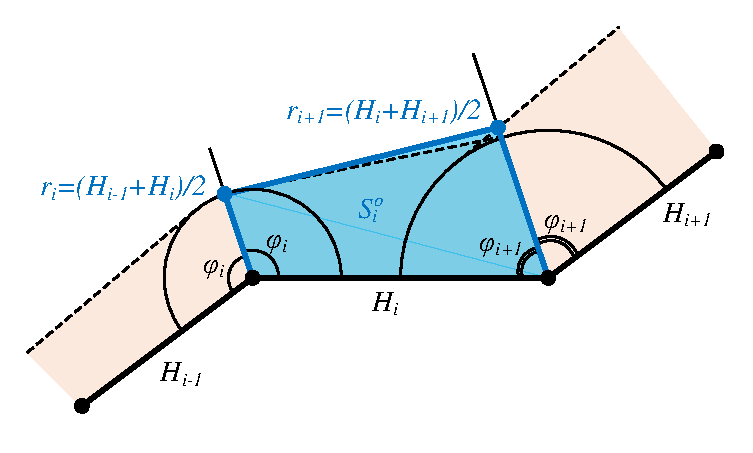
\includegraphics[width=0.6\textwidth]{fig/2dr_remesh_okrestnost.pdf}
\singlespacing
\captionstyle{center}\caption{Перестроение поверхности методом окрестностей.}
\label{fig:text_1_remesh_2d_okrestnost}
\end{figure}

Шар с центром в точке $C$ и радиуса $R$, обозначаемый как $Ball(C, R)$, будем определять как ГМТ $\overline{P}$, удовлетворяющих условию
\begin{equation}
	|\overline{P} - \overline{C}| \le R
\end{equation}

Сферу с центром в точке $C$ и радиуса $R$, представляющую собой поверхность шара $Ball(C, R)$, будем обозначать $Sphere(C, R)$.

\begin{definition}
Пусть дано некоторое ГМТ\label{abbr:gmt-2} $G$, на точках $P \in G$ которого определена неотрицательная функция $R: G \rightarrow \mathbb{R}_{\ge 0}$.
Тогда окрестностью $G$, заданной указанной функцией $R(P)$, будем называть ГМТ, определяемое следующим образом:
\begin{equation}
	O_R(G) = \{ P: \exists C \in G \implies P \in Ball(C, R(C)) \}
\end{equation}
\end{definition}

Окрестность ячейки или сетки несет смысл области распространения льда (ОРЛ\label{abbr:orl-1}), где функция $R(C)$ соотвествует радиусу распространения льда в точке $C$.
ОРЛ узла с номером $i$ будем считать сферу с центром в этом узле и радиусом $R_i = \frac{H_{i - 1} + H_i}{2}$.
ОРЛ ячейки является выпуклая оболочка ОРЛ двух инцидентных ей узлов.
Тогда ОРЛ сетки является объединение ОРЛ всех ее ячеек.
В качестве нового положения узла будем брать пересечение направления смещения узла и границы ОРЛ сетки, то есть ее окрестности.
Заметаемую $i$-ой ячейкой площадь при использовании метода окрестностей будем обозначать $S_i^o$, а абсолютное и относительное отклонения от целевой площади -- $\Delta_i^o = S_i^o - T_i$ и $\delta_i^o = \frac{\Delta_i^o}{T_i}$ соответственно.

%---------------------------------------------------------------------------------------------------

\subsection{Аналитические оценки точности}

Приведем аналитические оценки точности приближенных методов перестроения поверхностной расчетной сетки.
Оценки будем проводить для модельной расчетной сетки, которая удовлетворяет следующим требованиям.
Все ячейки сетки одинаковые и имеют длину $l$.
Для любой ячейки $AB$ и ее соседей $A_1A$ и $BB_1$ углы $\angle (\overline{BA}, \overline{AA_1})$ и $\angle (\overline{AB}, \overline{BB_1})$ являются постоянной величиной и равны $\alpha$ (см. рис.~\ref{fig:text_1_remesh_2d_theoretical}).
Пусть величины смещений ячеек $A_1A$, $AB$ и $BB_1$ равны $H_{i - 1}$, $H_i$ и $H_{i + 1}$ соответственно.

\subsubsection{Оценки точности для выпуклой сетки}

Сначала рассмотрим случай, когда сетка является выпуклой.

\begin{definition}
Поверхностная расчетная сетка называется выпуклой в некоторой ячейке $AB$, если из двух полуплоскостей, на которые прямая $AB$ разбивает плоскость, все смежные $AB$ ячейки лежат в одной полуплоскости, а внешняя нормаль $\overline{n}_{AB}^F$ направлена в другую полуплоскость.
\end{definition}

\begin{figure}[ht]
\centering
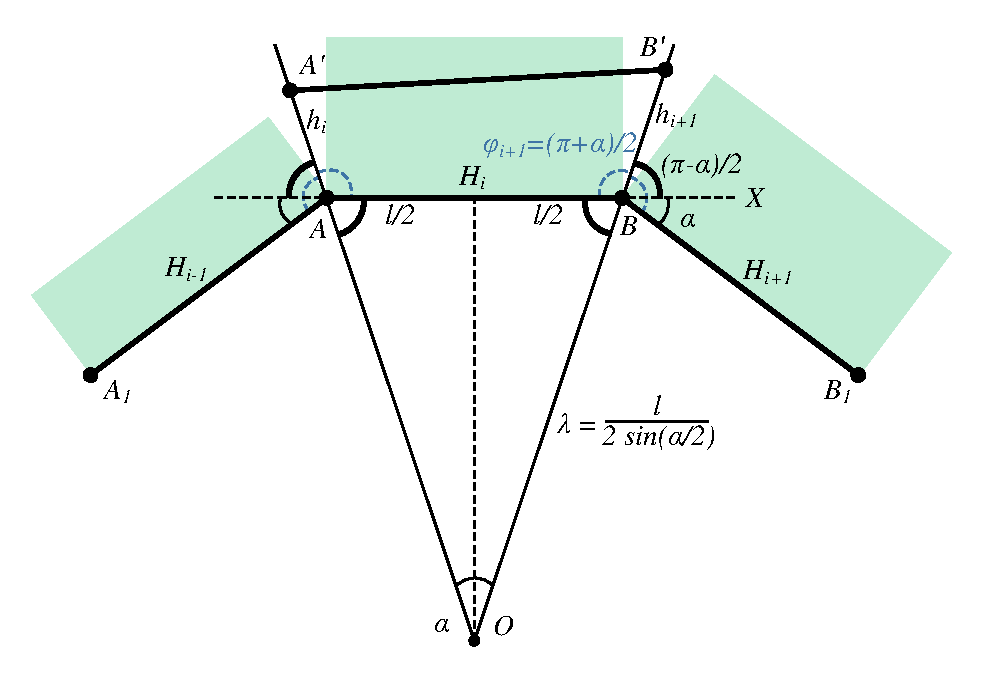
\includegraphics[width=0.8\textwidth]{fig/2dr_theoretical_convex.pdf}
\singlespacing
\captionstyle{center}\caption{Оценка приближенных методов перестроения выпуклой в ячейке $AB$ поверхностной расчетной сетки в двумерном случае.}
\label{fig:text_1_remesh_2d_theoretical}
\end{figure}

Для вычисления величин $\Delta$, $\delta$ необходимо вычислить площадь $S_i = S_{AA'B'B}$.
При использовании разных методов перестроения эта площадь будет различаться.

\begin{lemma}\label{lem:text_1_remesh2_vypukl_lemma}
Для поверхностной расчетной сетки, выпуклой в ячейке $F_i = AB$, при выполнении условия $\angle (\overline{BA}, \overline{AA_1}) = \angle (\overline{AB}, \overline{BB_1}) = \alpha$ (см. рис.~\ref{fig:text_1_remesh_2d_theoretical}) верно соотношение
\begin{equation}\label{eqn:text_1_remesh2_saa2b2b_gen}
S_i(h_i, h_{i + 1}) = \frac{1}{2} \sin \alpha \left( \lambda(h_i + h_{i+1}) + h_ih_{i+1} \right)
\end{equation}
где $\lambda = \frac{l}{2 \sin \frac{\alpha}{2}}$, $l = AB$, $h_i = AA'$, $h_{i + 1} = BB'$.
\end{lemma}

Так как рассматриваемая сетка выпуклая в ячейке $AB$, то лучи $A'A$ и $B'B$ пересекаются в некоторой точке $O$.
При этом треугольник $AOB$ равнобедренный, $\angle BAO = \angle ABO = \angle B'BX = \angle B'BB_1 - \alpha = \frac{\pi - \alpha}{2}$, $\phi_i = \phi_{i + 1} = \frac{\pi + \alpha}{2}$, $\angle AOB = \alpha$, откуда $OA = OB = \lambda = \frac{l}{2 \sin \frac{\alpha}{2}}$.
Далее выражаем площадь $S_i = S_{A'OB'} - S_{AOB}$, что после преобразования и дает требуемое соотношение \eqref{eqn:text_1_remesh2_saa2b2b_gen}.
$\blacksquare$\\

Далее будем рассматривать линейное изменение величины смещения ячеек сетки, то есть $H_i = H$, $H_{i - 1} = H - \Delta H$, $H_{i + 1} = H + \Delta H$.

Для перестроения методом прямоугольников имеем $h_i = H - \frac{1}{2} \Delta H$, $h_{i + 1} = H + \frac{1}{2} \Delta H$, откуда
\begin{equation}\label{eqn:text_1_remesh2_s_rect}
	S_i^r = \cos \frac{\alpha}{2} \left( lH + ( H^2 - \frac{1}{4} \Delta H^2) \sin \frac{\alpha}{2} \right)
\end{equation}

Теперь перейдем к вычислению $S_i^t$ для метода трапеций.
В методе трапеций мы должны представить целевые площади в ячейках $A_1A$, $AB$, $BB_1$ с помощью равнобоких трапеций, для которых известно одно из оснований (одинаково для всех ячеек и равно $l$), угол при этом основании (одинаковый для всех ячеек и равен $\phi = \frac{\pi + \alpha}{2}$, а также площади этих трапеций, равные $T_{i - 1} = l(H - \Delta H)$, $T_i = lH$ и $T_{i + 1} = l(H + \Delta H)$ соответственно.
На основании этих данных нам необходимо вычислить высоты трапеций, что можно сделать согласно \eqref{eqn:text_1_geo_prim_trapezium_h_from_s}.
Обозначим высоты этих трапеций:
\begin{equation}
	\begin{aligned}\label{eqn:text_1_remesh_2_Ht_vypukl}
		& H_{i - 1}^t = H^t\left(l(H - \Delta H), l, \frac{\pi + \alpha}{2}\right) \\ 
		& H_i^t = H^t\left(lH, l, \frac{\pi + \alpha}{2}\right) \\
		& H_{i + 1}^t = H^t\left(l(H + \Delta H), l, \frac{\pi + \alpha}{2}\right)
	\end{aligned}
\end{equation}

Тогда $h_i = \frac{H_{i - 1}^t + H_i^t}{2 \sin \phi_i} = \frac{H_{i - 1}^t + H_i^t}{2 \cos \frac{\alpha}{2}}$, $h_{i+1} = \frac{H_i^t + H_{i+1}^t}{2 \sin \phi_{i + 1}} = \frac{H_i^t + H_{i+1}^t}{2 \cos \frac{\alpha}{2}}$ и выражение \eqref{eqn:text_1_remesh2_saa2b2b_gen} для $S_i^t$ принимает следующий вид:
\begin{equation}\label{eqn:text_1_remesh2_trap}
	S_i^t = \frac{1}{4} \left( (H_{i - 1}^t + 2 H_i^t + H_{i + 1}^t)l + (H_{i - 1}^t + H_i^t) (H_i^t + H_{i+1}^t) \tg \frac{\alpha}{2} \right)
\end{equation}

Для получения аналитической оценки точности для метода окрестностей в случае выпуклой сетки рассмотрим следующее вспомогательное утверждение.

\begin{figure}[ht]
\centering
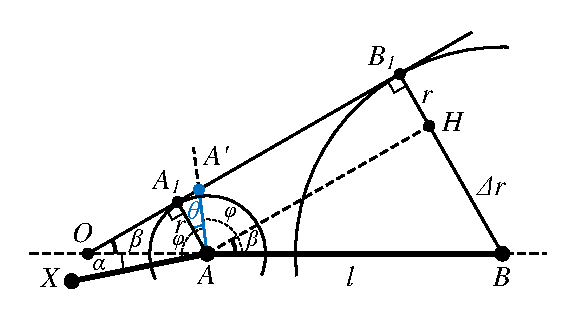
\includegraphics[width=0.7\textwidth]{fig/2dr_accuracy_okrestnost.pdf}
\singlespacing
\captionstyle{center}\caption{Вычисление смещения узла в методе окрестностей для выпуклой расчетной сетки.}
\label{fig:text_1_remesh_2d_accuracy_okrestnost}
\end{figure}

\begin{lemma}\label{lem:text_1_remesh_2d_accuracy_okrestnost}
Пусть $AB = l$, ниже прямой $AB$ расположена точка $X$ такая, что $\angle (\overline{AX}, \overline{BA}) = \alpha$.
Пусть построены две окружности с центрами в точках $A$ и $B$ и с радиусами $r$ и $r + \Delta r$ соответственно.
Для построенных окружностей построена выпуклая оболочка, состоящая из дуг этих окружностей, а также отрезков общих касательных (точки касания общей касательной построенных окружностей, лежащие выше прямой $AB$, обозначим $A_1$ и $B_1$ соответственно).
Пусть на этой выпуклой оболочке -- на окружности с центром в точке $A$, либо на отрезке $A_1B_1$ -- лежит точка $A'$ такая, что $\angle XAA' = \angle BAA' = \phi$, $AA' = h$, тогда 
\begin{equation}
	\begin{cases}\label{eqn:text_1_remesh_2d_okr_h}
		h = r, \  \sin \frac{\alpha}{2} > \frac{\Delta r}{l}, \\
		h(\alpha, l, r, \Delta r) = \frac{r}{\cos \left( \arcsin \frac{\Delta r}{l} - \frac{\alpha}{2} \right)}, \  \sin \frac{\alpha}{2} \le \frac{\Delta r}{l}
	\end{cases}
\end{equation}
\end{lemma}

Если $\Delta r \le 0$, то точка $A'$ находится на окружности с центром в точке $A$, то есть $h = r$.

Рассмотрим случай, когда $A'$ находится на отрезке $A_1B_1$, в этом случае $\Delta r > 0$.
Через точку $A$ проведем прямую, параллельную $A_1B_1$, до пересечения с $BB_1$ в точке $H$.
Тогда $\angle B_1OB = \angle HAB = \beta = \arcsin \frac{\Delta r}{l}$.
Так как $\angle A'AB = \phi = \frac{\pi + \alpha}{2}$, а $\angle OAA_1 + \angle A_1AA' + \phi = \pi$, то $\theta = \angle A_1AA' = \beta - \frac{\alpha}{2}$.

Таким образом, условие нахождения точки $A'$ на отрезке $A_1B_1$ равносильно $\theta \ge 0$.
То есть при $\theta < 0$, получаем $h = r$, а при $\theta \ge 0$ значение $h$ можно выразить из прямоугольного треугольника $AA'A_1$.
$\blacksquare$\\

Используя лемму~\ref{lem:text_1_remesh_2d_accuracy_okrestnost}, для метода окрестностей можно выразить $S_i^o$ из \eqref{eqn:text_1_remesh2_saa2b2b_gen} подставив туда выражения для $h_i$ и $h_{i + 1}$ из \eqref{eqn:text_1_remesh_2d_okr_h}:
\begin{equation}
	\begin{aligned}
	& h_i = h \left( \alpha, l, H - \frac{1}{2}\Delta H, \Delta H \right) \\
	& h_{i + 1} = h \left( \alpha, l, H + \frac{1}{2}\Delta H, \Delta H \right)
	\end{aligned}
\end{equation}

\subsubsection{Оценки точности для вогнутой сетки}

Теперь рассмотрим случай вогнутой сетки, представленный на рис.~\ref{fig:text_1_remesh_2d_theoretical_concave}.

\begin{definition}
Поверхностная расчетная сетка называется вогнутой в некоторой ячейке $AB$, если из двух полуплоскостей, на которые прямая $AB$ разбивает плоскость, все смежные $AB$ ячейки лежат в одной полуплоскости, и внешняя нормаль $\overline{n}_{AB}^F$ направлена в ту же полуплоскость.
\end{definition}

\begin{figure}[ht]
\centering
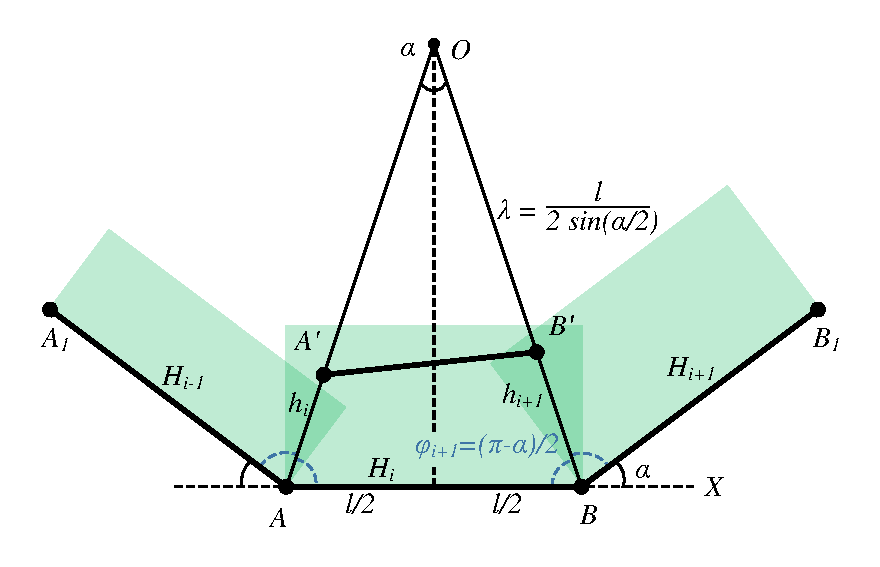
\includegraphics[width=0.8\textwidth]{fig/2dr_theoretical_concave.pdf}
\singlespacing
\captionstyle{center}\caption{Оценка приближенных методов перестроения вогнутой в ячейке $AB$ поверхностной расчетной сетки в двумерном случае.}
\label{fig:text_1_remesh_2d_theoretical_concave}
\end{figure}

\begin{lemma}
Для поверхностной расчетной сетки, вогнутой в ячейке $F_i = AB$, при выполнении условия $\angle (\overline{BA}, \overline{AA_1}) = \angle (\overline{AB}, \overline{BB_1}) = \alpha$ (см. рис.~\ref{fig:text_1_remesh_2d_theoretical_concave}) верно соотношение
\begin{equation}\label{eqn:text_1_remesh2_saa2b2b_gen2}
S_i = \frac{1}{2} \sin \alpha \left( \lambda(h_i + h_{i+1}) - h_ih_{i+1} \right)
\end{equation}
где $\lambda = \frac{1}{2 \sin \frac{\alpha}{2}}$, $l = AB$, $h_i = AA'$, $h_{i + 1} = BB'$, при этом формула \eqref{eqn:text_1_remesh2_saa2b2b_gen2} применима при выполнении хотя бы одного из условий $h_i \le \lambda$, $h_{i+1} \le \lambda$.
\end{lemma}

Вычисления производятся аналогично лемме~\ref{lem:text_1_remesh2_vypukl_lemma}, с той лишь разницей, что $S_i = S_{AOB} - S_{A'OB'}$, откуда имеем выражение \eqref{eqn:text_1_remesh2_saa2b2b_gen2}.

Выполнение хотя бы одного из условий $h_i \le \lambda$, $h_{i+1} \le \lambda$ необходимо для предотвращения самопересечения сетки.
$\blacksquare$\\

Для перестроения методом прямоугольников и методом трапеций в случае вогнутой сетки получим формулы, аналогичные \eqref{eqn:text_1_remesh2_s_rect}, \eqref{eqn:text_1_remesh_2_Ht_vypukl} и \eqref{eqn:text_1_remesh2_trap}:
\begin{equation}\label{eqn:text_1_remesh2_s_rect_vogn}
	S_i^r = \cos \frac{\alpha}{2} \left( lH - ( H^2 - \frac{1}{4} \Delta H^2 ) \sin \frac{\alpha}{2} \right) \\
\end{equation}
\begin{equation}\label{eqn:text_1_remesh_2_Ht_vogn}
	\begin{aligned}
	& H_{i - 1}^t = H^t\left(l(H - \Delta H), l, \frac{\pi - \alpha}{2}\right) \\ 
	& H_i^t = H^t\left(lH, l, \frac{\pi - \alpha}{2}\right) \\
	& H_{i + 1}^t = H^t\left(l(H + \Delta H), l, \frac{\pi - \alpha}{2}\right)
	\end{aligned}
\end{equation}
\begin{equation}\label{eqn:text_1_remesh2_trap_vogn}
	S_i^t = \frac{1}{4} \left( (H_{i - 1}^t + 2 H_i^t + H_{i + 1}^t)l - (H_{i - 1}^t + H_i^t) (H_i^t + H_{i+1}^t) \tg \frac{\alpha}{2} \right)
\end{equation}

Заметим, что формулы \eqref{eqn:text_1_remesh2_s_rect_vogn} -- \eqref{eqn:text_1_remesh2_trap_vogn} идентичны формулам \eqref{eqn:text_1_remesh2_s_rect} -- \eqref{eqn:text_1_remesh2_trap} с учетом знака $\alpha$, поэтому формулы \eqref{eqn:text_1_remesh2_s_rect} -- \eqref{eqn:text_1_remesh2_trap} применимы как для выпуклой расчетной сетки (в этом случае используется положительное значение угла $\alpha$), так и для вогнутой сетки (в этом случае используем формулы \eqref{eqn:text_1_remesh2_s_rect} -- \eqref{eqn:text_1_remesh2_trap} с отрицательным значением угла $\alpha$).

Для получения аналитической оценки точности для метода окрестностей в случае вогнутой сетки рассмотрим следующее вспомогательное утверждение, аналогичное лемме~\ref{lem:text_1_remesh_2d_accuracy_okrestnost}.

\begin{figure}[ht]
\centering
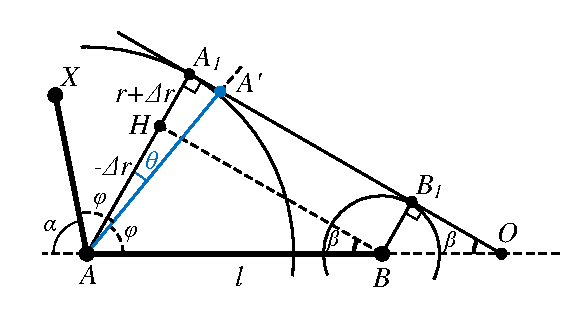
\includegraphics[width=0.7\textwidth]{fig/2dr_accuracy_okrestnost2.pdf}
\singlespacing
\captionstyle{center}\caption{Вычисление смещения узла в методе окрестностей для вогнутой сетки.}
\label{fig:text_1_remesh_2d_accuracy_okrestnost}
\end{figure}

\begin{lemma}\label{lem:text_1_remesh_2d_accuracy_okrestnost2}
Пусть $AB = l$, выше прямой $AB$ расположена точка $X$ такая, что $\angle (\overline{AX}, \overline{BA}) = \alpha$.
Пусть построены две окружности с центрами в точках $A$ и $B$ и с радиусами $r$ и $r + \Delta r$ соответственно.
Для построенных окружностей построена выпуклая оболочка, состоящая из дуг этих окружностей, а также отрезков общих касательных (точки касания общей касательной построенных окружностей, лежащие выше прямой $AB$, обозначим $A_1$ и $B_1$ соответственно).
Пусть на этой выпуклой оболочке -- на окружности с центром в точке $A$ либо на отрезке $A_1B_1$ -- лежит точка $A'$ такая, что $\angle XAA' = \angle BAA' = \phi$, $AA' = h$, тогда 
\begin{equation}
	\begin{cases}\label{eqn:text_1_remesh_2d_okr_h2}
		h = r, \ \sin \frac{\alpha}{2} < \frac{-\Delta r}{l}, \\
		h(\alpha, l, r, \Delta r) = \frac{r}{\cos \left( \frac{\alpha}{2} - \arcsin \frac{-\Delta r}{l} \right)}, \ \sin \frac{\alpha}{2} \ge \frac{-\Delta r}{l}
	\end{cases}
\end{equation}
\end{lemma}

Если $\Delta r \ge 0$, то точка $A'$ находится на отрезке $A_1B_1$.

Рассмотрим случай, когда $A'$ находится на отрезке $A_1B_1$, и $\Delta r < 0$.
Через точку $B$ проведем прямую, параллельную $A_1B_1$, до пересечения с $AA_1$ в точке $H$.
Тогда $\angle A_1OA = \angle HBA = \beta = \arcsin \frac{-\Delta r}{l}$.
Так как $\angle A'AB = \phi = \frac{\pi - \alpha}{2}$, то $\theta = \angle A_1AA' = \angle A_1AO - \phi = \frac{\alpha}{2} - \beta$.

Таким образом, условие нахождения точки $A'$ на отрезке $A_1B_1$ равносильно $\theta \ge 0$.
То есть при $\theta < 0$, получаем $h = r$, а при $\theta \ge 0$ значение $h$ можно выразить из прямоугольного треугольника $AA'A_1$.
$\blacksquare$\\

Используя лемму~\ref{lem:text_1_remesh_2d_accuracy_okrestnost2}, для метода окрестностей можно выразить $S_i^o$ из \eqref{eqn:text_1_remesh2_saa2b2b_gen2} подставив туда выражения для $h_i$ и $h_{i + 1}$ из \eqref{eqn:text_1_remesh_2d_okr_h2}:
\begin{equation}
	\begin{aligned}
	& h_i = \max \left( h \left( \alpha, l, H - \frac{3}{2}\Delta H, \Delta H \right), h \left( \alpha, l, H - \frac{1}{2}\Delta H, \Delta H \right) \right) \\
	& h_{i + 1} = \max \left( h \left( \alpha, l, H - \frac{1}{2}\Delta H, \Delta H \right), h \left( \alpha, l, H + \frac{1}{2}\Delta H, \Delta H \right) \right)
	\end{aligned}
\end{equation}

\subsubsection{Анализ оценок точности}

Используя полученные в предыдущем разделе соотношения для $S_i^r$, $S_i^t$, $S_i^o$, проанализируем зависимости величин $\delta_i^r$, $\delta_i^t$, $\delta_i^o$ от $\alpha$ и $\frac{\Delta H}{l}$, при этом будем использовать фиксированную величину $H = \frac{l}{2}$ (см. рис.~\ref{fig:text_1_remesh_3d_main_chart}).

\begin{figure}[ht]
\centering
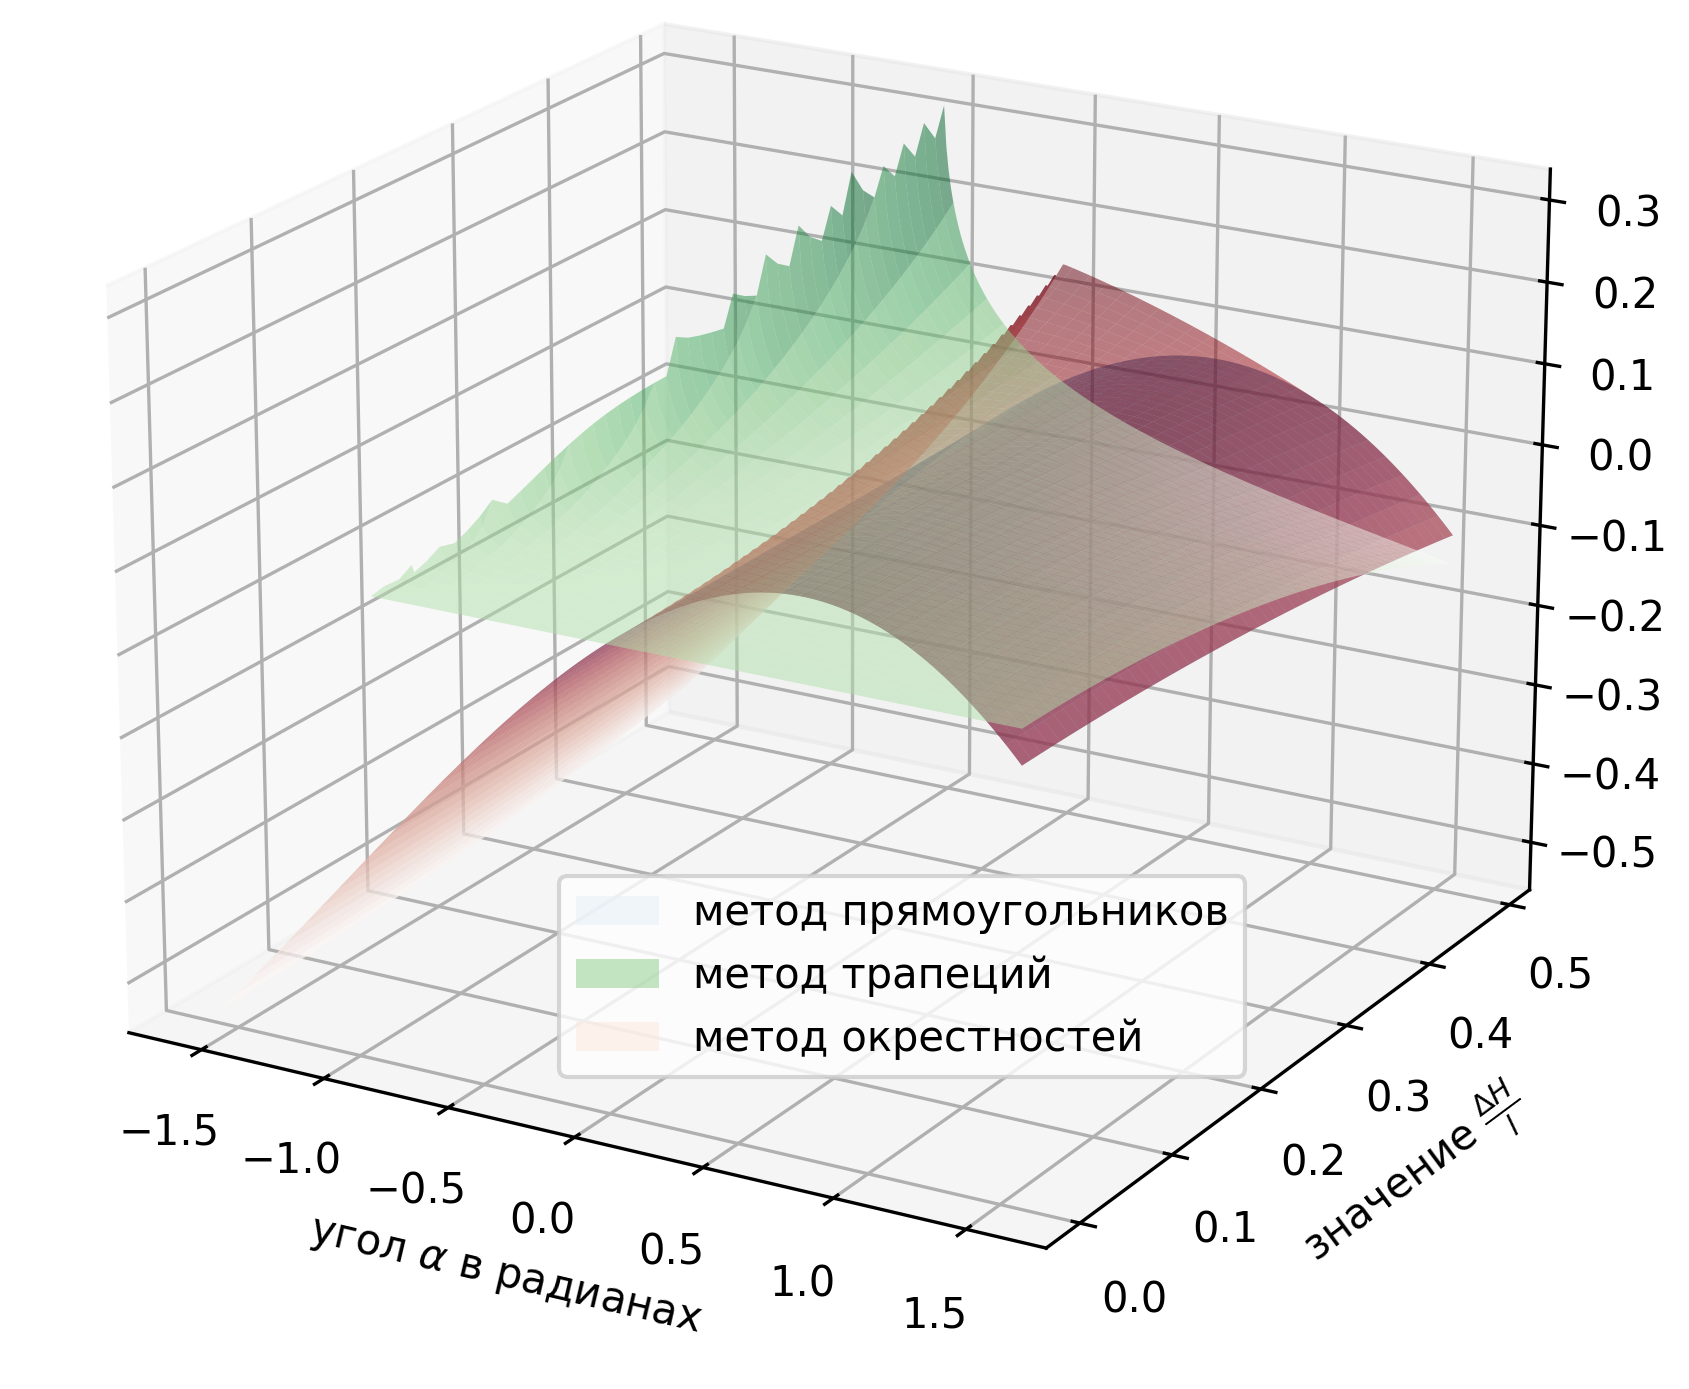
\includegraphics[width=0.8\textwidth]{fig/2dr_remesh_3d_chart.png}
\singlespacing
\captionstyle{center}\caption{Графики поверхностей $\delta_i^r(\alpha, \frac{\Delta H}{l})$, $\delta_i^t(\alpha, \frac{\Delta H}{l})$, $\delta_i^o(\alpha, \frac{\Delta H}{l})$ при фиксированном значении $H = \frac{l}{2}$.}
\label{fig:text_1_remesh_3d_main_chart}
\end{figure}

Анализируя полученные зависимости, графики которых приведены на рис.~\ref{fig:text_1_remesh_3d_main_chart}, можно отметить, что при $\Delta H = 0$ метод трапеций абсолютно точен.
Также отметим, что при малых значениях $\Delta H$ отклонения $\delta_i^r$ и $\delta_i^o$ практически совпадают.

Построим дополнительно два графика зависимостей $\delta_i^r$, $\delta_i^t$, $\delta_i^o$ от $\frac{\Delta H}{l}$ при фиксированных значениях $\alpha = 0,5$ (для выпуклой сетки) и $\alpha = -0,5$ (для вогнутой сетки) (см. рис.~\ref{fig:text_1_remesh_fix_alfa_chart}).
Из рисунка видно, что метод трапеций перестроения поверхности при небольших значениях $\frac{\Delta H}{l}$ наиболее точен, а точность методов прямоугольников и окрестностей достаточно близки.

\begin{figure}[ht]
\centering
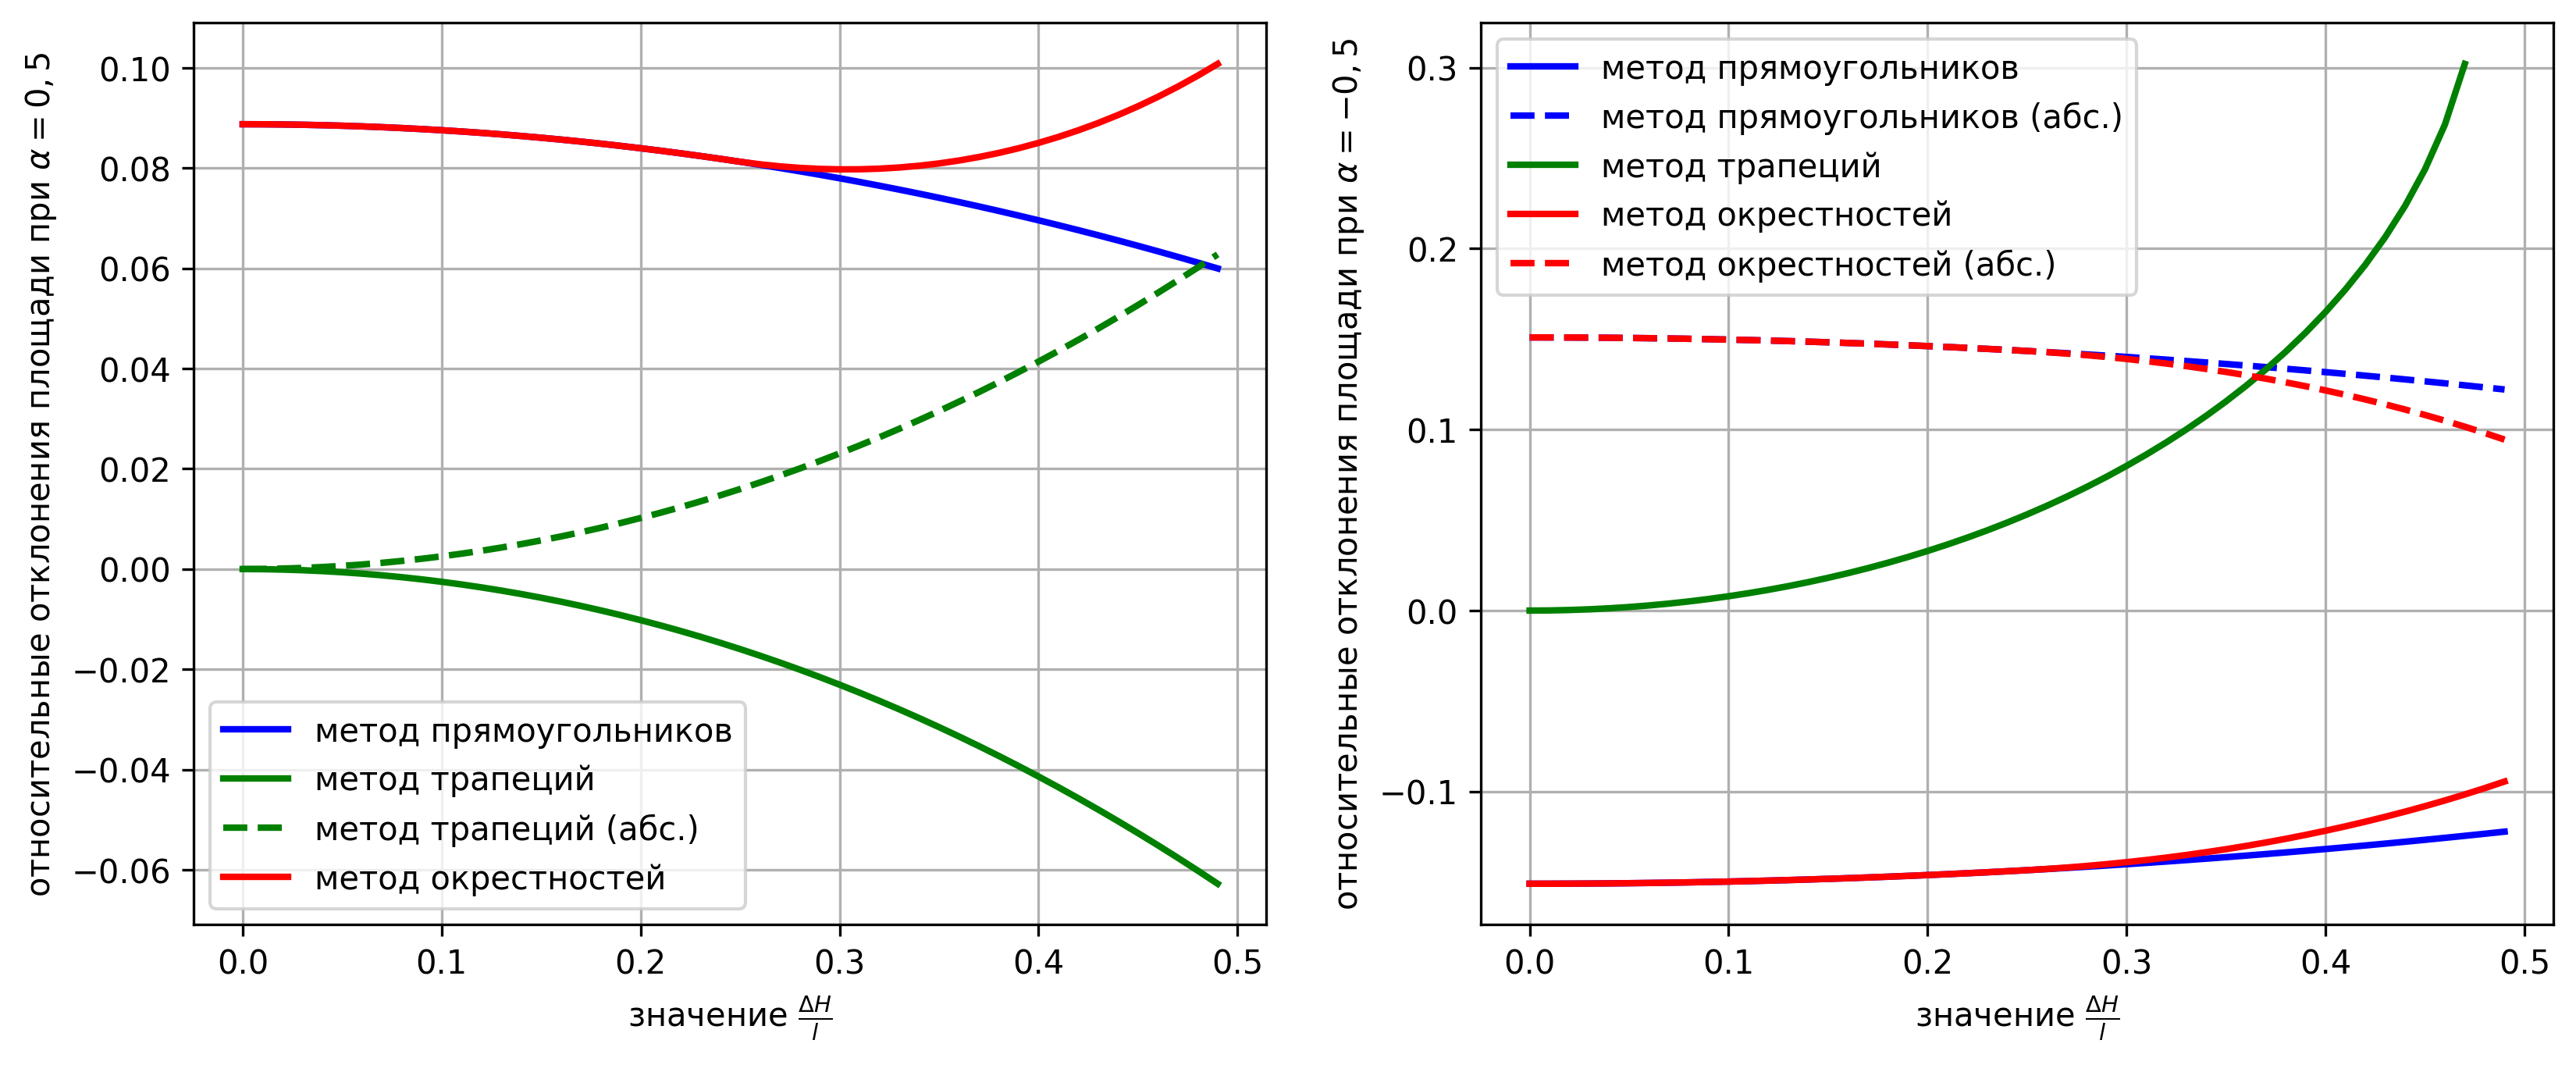
\includegraphics[width=1.0\textwidth]{fig/2dr_remesh_fix_alfa_chart.png}
\singlespacing
\captionstyle{center}\caption{Графики зависимостей $\delta_i^r(\frac{\Delta H}{l})$, $\delta_i^t(\frac{\Delta H}{l})$, $\delta_i^o(\frac{\Delta H}{l})$ при фиксированных значениях $\alpha = 0,5$ (слева) и $\alpha = -0,5$ (справа).}
\label{fig:text_1_remesh_fix_alfa_chart}
\end{figure}

%---------------------------------------------------------------------------------------------------

\subsection{Оценки сглаживания острых пиков и впадин}

В процессе перестроения поверхностной расчетной сетки могут возникать мелкие дефекты, такие как острые пики (если значение $\phi_i$ близко к $\pi$) и впадины (если значение $\phi_i$ близко к нулю).

Приведем оценки сглаживания острых пиков и впадин для рассмотренных методов перестроения (методы прямоугольников, трапеций и окрестностей).
Для этого будем рассматривать расчетную сетку с одинаковыми ячейками-отрезками длины $l$.

Для оценки сглаживания острых пиков будем считать, что сетка является абсолютно плоской за исключением двух соседних ячеек, которые образуют острый пик с углом $2 \alpha$ (см. рис.~\ref{fig:text_1_remesh_2d_peak_cavern_general} слева).
Аналогично для оценки сглаживания впадин будем считать, что сетка является абсолютно плоской за исключением двух соседних ячеек, которые образуют впадину с углом $2 \alpha$ (см. рис.~\ref{fig:text_1_remesh_2d_peak_cavern_general} справа)

\begin{figure}[ht]
\centering
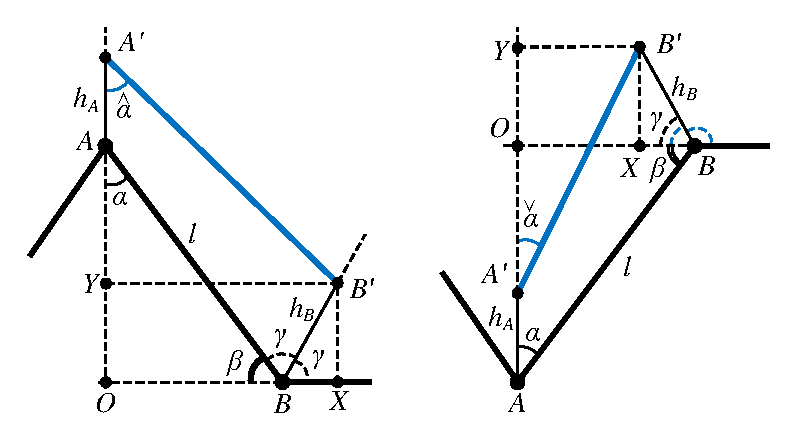
\includegraphics[width=0.8\textwidth]{fig/2dr_peak_cavern_general.pdf}
\singlespacing
\captionstyle{center}\caption{Оценка сглаживания угла при остром пике (слева) \\ и при впадине (справа).}
\label{fig:text_1_remesh_2d_peak_cavern_general}
\end{figure}

\subsubsection{Получение аналитических оценок сглаживания дефектов}

Во всех трех методах (прямоугольников, трапеций и окрестностей) направления смещения узлов совпадают (и лежат на биссектрисах углов, образованных соседними ячейками), поэтому будем рассматривать задачу сглаживания угла при остром пике и при впадине для произвольных смещений узлов $A$ и $B$.
Для этого докажем следующие леммы.

\begin{lemma}\label{lem:text_1_peak_smooth}
При перемещении узлов $A$ и $B$ -- узлов одной из сторон острого пика -- вдоль биссектрис углов, образованных инцидентными ячейками, на расстояния $h_A$ и $h_B$ соответственно (см. рис.~\ref{fig:text_1_remesh_2d_peak_cavern_general} слева) значение сглаженного угла $\hat{\alpha} = \angle OA'B'$ выражается через $\alpha = \angle OAB$ и $\gamma = \frac{\pi}{4} + \frac{\alpha}{2}$ следующим образом:
\begin{equation}\label{eqn:text_1_envelope_alpha1_peak}
\hat{\alpha}(h_A, h_B) = \arctg \frac{l \sin \alpha + h_B \cos \gamma}{l \cos \alpha + h_A - h_B \sin \gamma}	
\end{equation}
\end{lemma}

Выразим через $\alpha$ остальные углы: $\beta = \angle OBA = \frac{\pi}{2} - \alpha$, $\gamma = \angle ABB' = \angle XBB' = \frac{\pi}{4} + \frac{\alpha}{2}$.
Через углы $\alpha$ и $\gamma$ находим $OA = l \cos \alpha$, $OB = l \sin \alpha$, $BX = h_B \cos \gamma$, $B'X = h_B \sin \gamma = OY$, откуда получаем $YB' = OB + BX = l \sin \alpha + h_B \cos \gamma$, $YA' = OA + AA' - OY = l \cos \alpha + h_A - h_B \sin \gamma$, откуда получаем $\hat{\alpha}(h_A, h_B) = \arctg \frac{YB'}{YA'}$, что приводит к \eqref{eqn:text_1_envelope_alpha1_peak}.
$\blacksquare$\\

\begin{lemma}\label{lem:text_1_cavern_smooth}
При перемещении узлов $A$ и $B$ -- узлов одной из сторон впадины -- вдоль биссектрис углов, образованных инцидентными ячейками, на расстояния $h_A \le AO$ и $h_B$ соответственно (см. рис.~\ref{fig:text_1_remesh_2d_peak_cavern_general} справа) значение сглаженного угла $\check{\alpha} = \angle OA'B'$ выражается через $\alpha = \angle OAB$ и $\gamma = \frac{\pi}{4} + \frac{\alpha}{2}$ следующим образом:
\begin{equation}\label{eqn:text_1_envelope_alpha1_cavern}
\check{\alpha}(h_A, h_B) = \arctg \frac{l \sin \alpha - h_B \cos \gamma}{l \cos \alpha - h_A + h_B \sin \gamma}
\end{equation}
при ограничениях на угол $\alpha$
\begin{equation}\label{eqn:text_1_envelope_alpha1_cavern2}
\arcsin \frac{h_B \left( \sqrt{8 l^2 + h_B^2} - h_B \right)}{4 l^2} \le \alpha \le \arccos \frac{h_A}{l}
\end{equation}
\end{lemma}

Выразим через $\alpha$ остальные углы: $\beta = \angle OBA = \frac{\pi}{2} - \alpha$, $\gamma = \angle OBB' = \frac{\pi}{4} + \frac{\alpha}{2}$.
Через углы $\alpha$ и $\gamma$ находим $OA = l \cos \alpha$, $OB = l \sin \alpha$, $BX = h_B \cos \gamma$, $B'X = h_B \sin \gamma = OY$, откуда получаем $YB' = OB - BX = l \sin \alpha - h_B \cos \gamma$, $YA' = OA - AA' + OY = l \cos \alpha - h_A + h_B \sin \gamma$, откуда получаем $\check{\alpha}(h_A, h_B) = \arctg \frac{YB'}{YA'}$, что приводит к \eqref{eqn:text_1_envelope_alpha1_cavern}.

Рассмотрим дополнительные условия применимости формулы \eqref{eqn:text_1_envelope_alpha1_cavern}.

Условие $h_A \le AO$ равносильно $\alpha \le \arccos \frac{h_A}{l}$.

Требованием на отсутствие самопересечения сетки является условие $BX \le OB$, то есть, то есть $h_B \cos \gamma \le l \sin \alpha$.
Подставляя явное выражение для $\cos \gamma$, получим
\begin{equation}
	h_B \frac{1}{\sqrt{2}} \left( \cos \frac{\alpha}{2} - \sin \frac{\alpha}{2} \right) \le l \sin \alpha
\end{equation}

Так как $\alpha < \frac{\pi}{2}$, то обе части неравенства положительные, поэтому возведем их в квадрат, и после преобразований получим
\begin{equation}\label{eqn:text_1_envelope_find_alpha3}
	1 - \sin \alpha \le 2 \left( \frac{l}{h_B} \right)^2 \sin^2 \alpha
\end{equation}

Введя обозначение $p = 2 \left( \frac{l}{h_B} \right)^2$ и решая квадратное неравенство \eqref{eqn:text_1_envelope_find_alpha3} относительно $\sin \alpha$, получим условие $\alpha \ge \arcsin \frac{\sqrt{4p + 1} - 1}{2p}$, что в сококупности с условием $\alpha \le \arccos \frac{h_A}{l}$ приводит к \eqref{eqn:text_1_envelope_alpha1_cavern2}.
$\blacksquare$\\

\begin{figure}[ht]
\centering
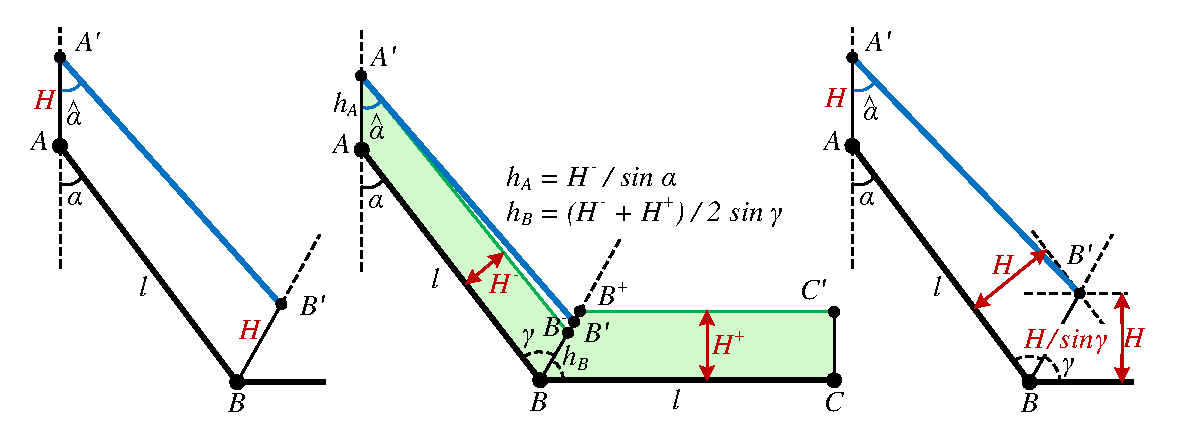
\includegraphics[width=1.0\textwidth]{fig/2dr_peak_methods.pdf}
\singlespacing
\captionstyle{center}\caption{Сглаживание пика при методах прямоугольников (слева), трапеций (в центре), окрестностей (справа).}
\label{fig:text_1_remesh_2d_peak_methods}
\end{figure}

\begin{figure}[ht]
\centering
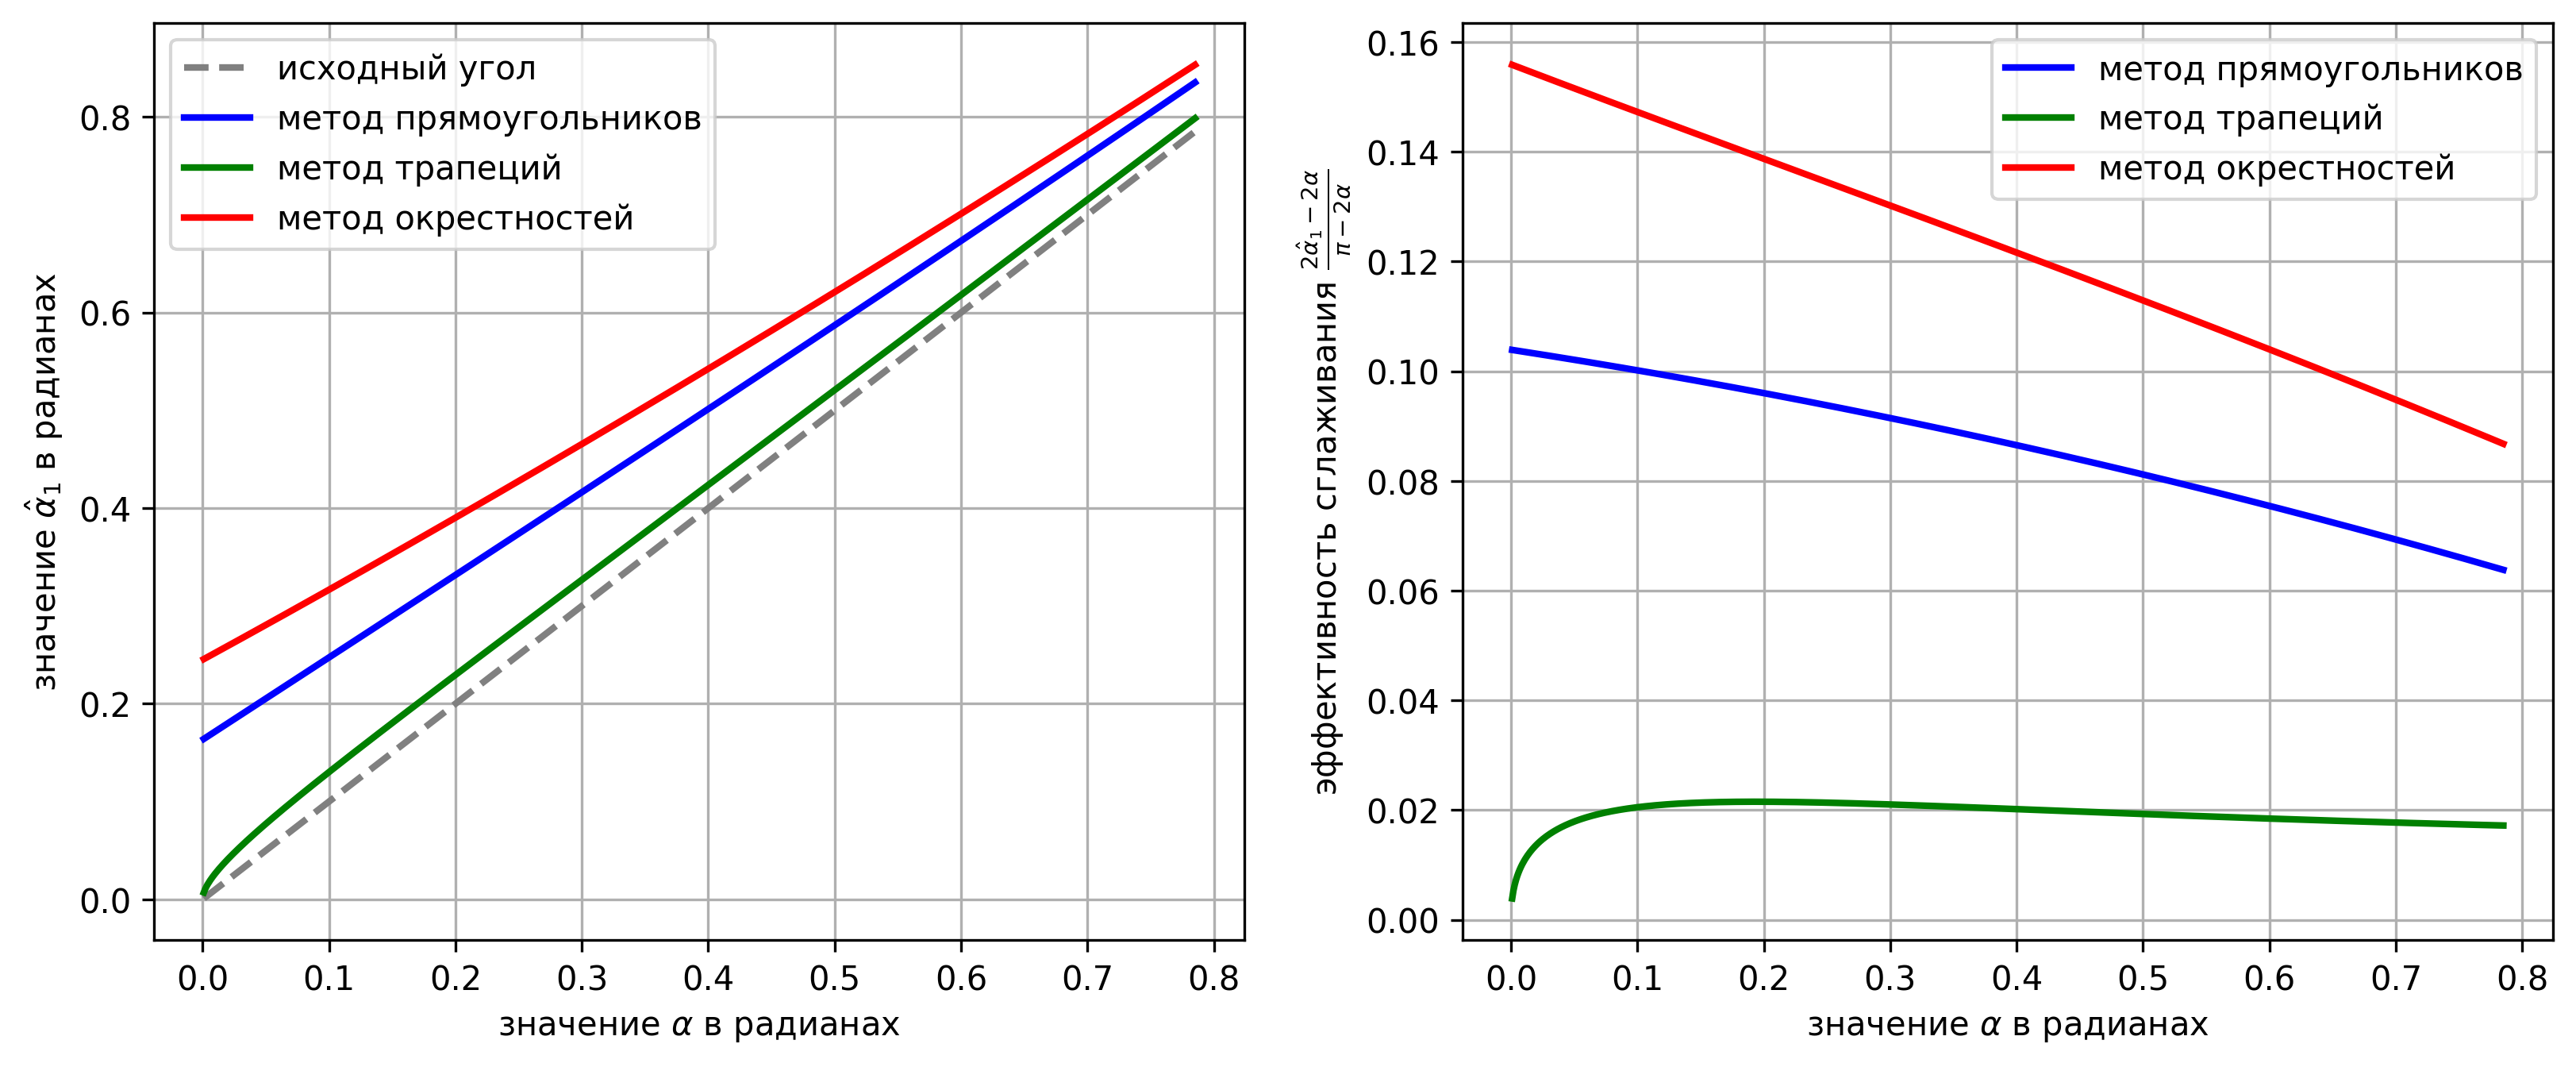
\includegraphics[width=1.0\textwidth]{fig/2dr_peak_methods_chart.png}
\singlespacing
\captionstyle{center}\caption{Сравнение сглаживания острого пика для методов прямоугольников, трапеций и окрестностей.}
\label{fig:text_1_remesh_2d_peak_methods_chart}
\end{figure}

\subsubsection{Анализ оценок сглаживания острых пиков}

На основе Леммы~\ref{lem:text_1_peak_smooth} получим оценки сглаживания угла при остром пике при условии постоянного значения $H$ во всех ячейках сетки.

Для метода прямоугольников имеем $h_A = h_B = H$ (см. рис~\ref{fig:text_1_remesh_2d_peak_methods} слева).

Для метода трапеций необходимо сначала найти высоты двух трапеций $AA'B^{-}B$ и $CC'B^{+}B$ с рис.~\ref{fig:text_1_remesh_2d_peak_methods} в центре из условия равенства площадей этих трапеций значению $lH$.
Высоты этих трапеций $H^{-}$ и $H^{+}$ получаются из \eqref{eqn:text_1_geo_prim_aa1b1b} с помощью решения квадратного уравнения.
Тогда $h_A = \frac{H^{-}}{\sin \alpha}$, $h_B = \frac{H^{-} + H^{+}}{2 \sin \gamma}$.
Из выражения для $h_A$ видно, что при малых значениях $\alpha$ смещение $h_A$ неконтролируемо возрастает.

В случае метода окрестностей $h_A = H$,  $h_B = \frac{H}{\sin \gamma}$ (см. рис.~\ref{fig:text_1_remesh_2d_peak_methods} справа).

На рис.~\ref{fig:text_1_remesh_2d_peak_methods_chart} приведены графики сравнения методов прямоугольников, трапеций и окрестностей в применении к сглаживанию острых пиков.
При этом используется фиксированная величина смещения ячейки $H = \frac{l}{4}$.
На графике слева показана зависимость изменения сглаженного угла $\hat{\alpha}$ от $\alpha$.
На графике справа показана эффективность сглаживания, выраженная формулой $\frac{\check{\alpha} - \alpha}{\frac{\pi}{2} - \alpha} = \frac{2 \check{\alpha} - 2 \alpha}{\pi - 2 \alpha}$ (значение 1 означает полное сглаживание пика до угла $\hat{\alpha} = \frac{\pi}{2}$).

Можно отметить, что наиболее эффективное сглаживание угла $\alpha$ обеспечивает метод окрестностей, а наименее эффективное -- метод трапеций.
Дополнительно заметим, что использование метода трапеций для малых углов $\alpha$ приводит к неконтролируемому росту $h_A$, что делает применение этого метода неприемлемым.

\subsubsection{Анализ оценок сглаживания впадин}

\begin{figure}[ht]
\centering
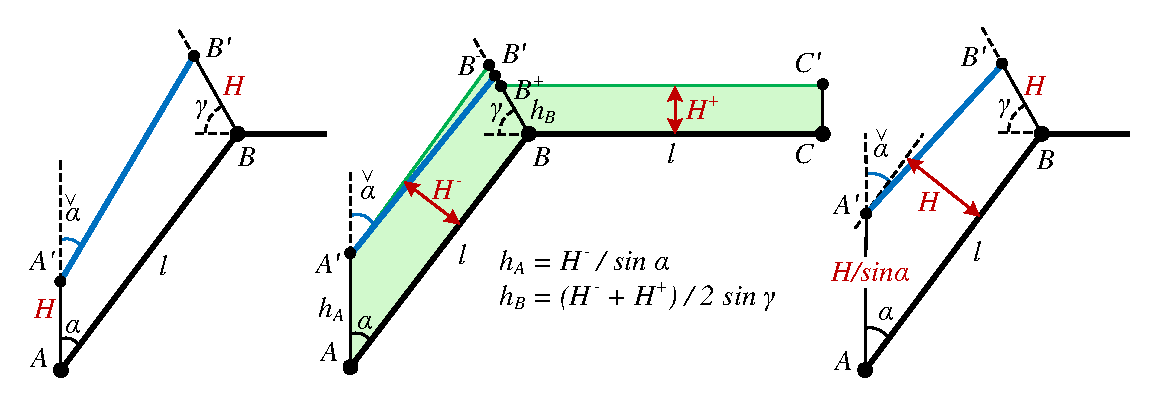
\includegraphics[width=1.0\textwidth]{fig/2dr_cavern_methods.pdf}
\singlespacing
\captionstyle{center}\caption{Сглаживание впадины при методах прямоугольников (слева), трапеций (в центре), окрестностей (справа).}
\label{fig:text_1_remesh_2d_cavern_methods}
\end{figure}

\begin{figure}[ht]
\centering
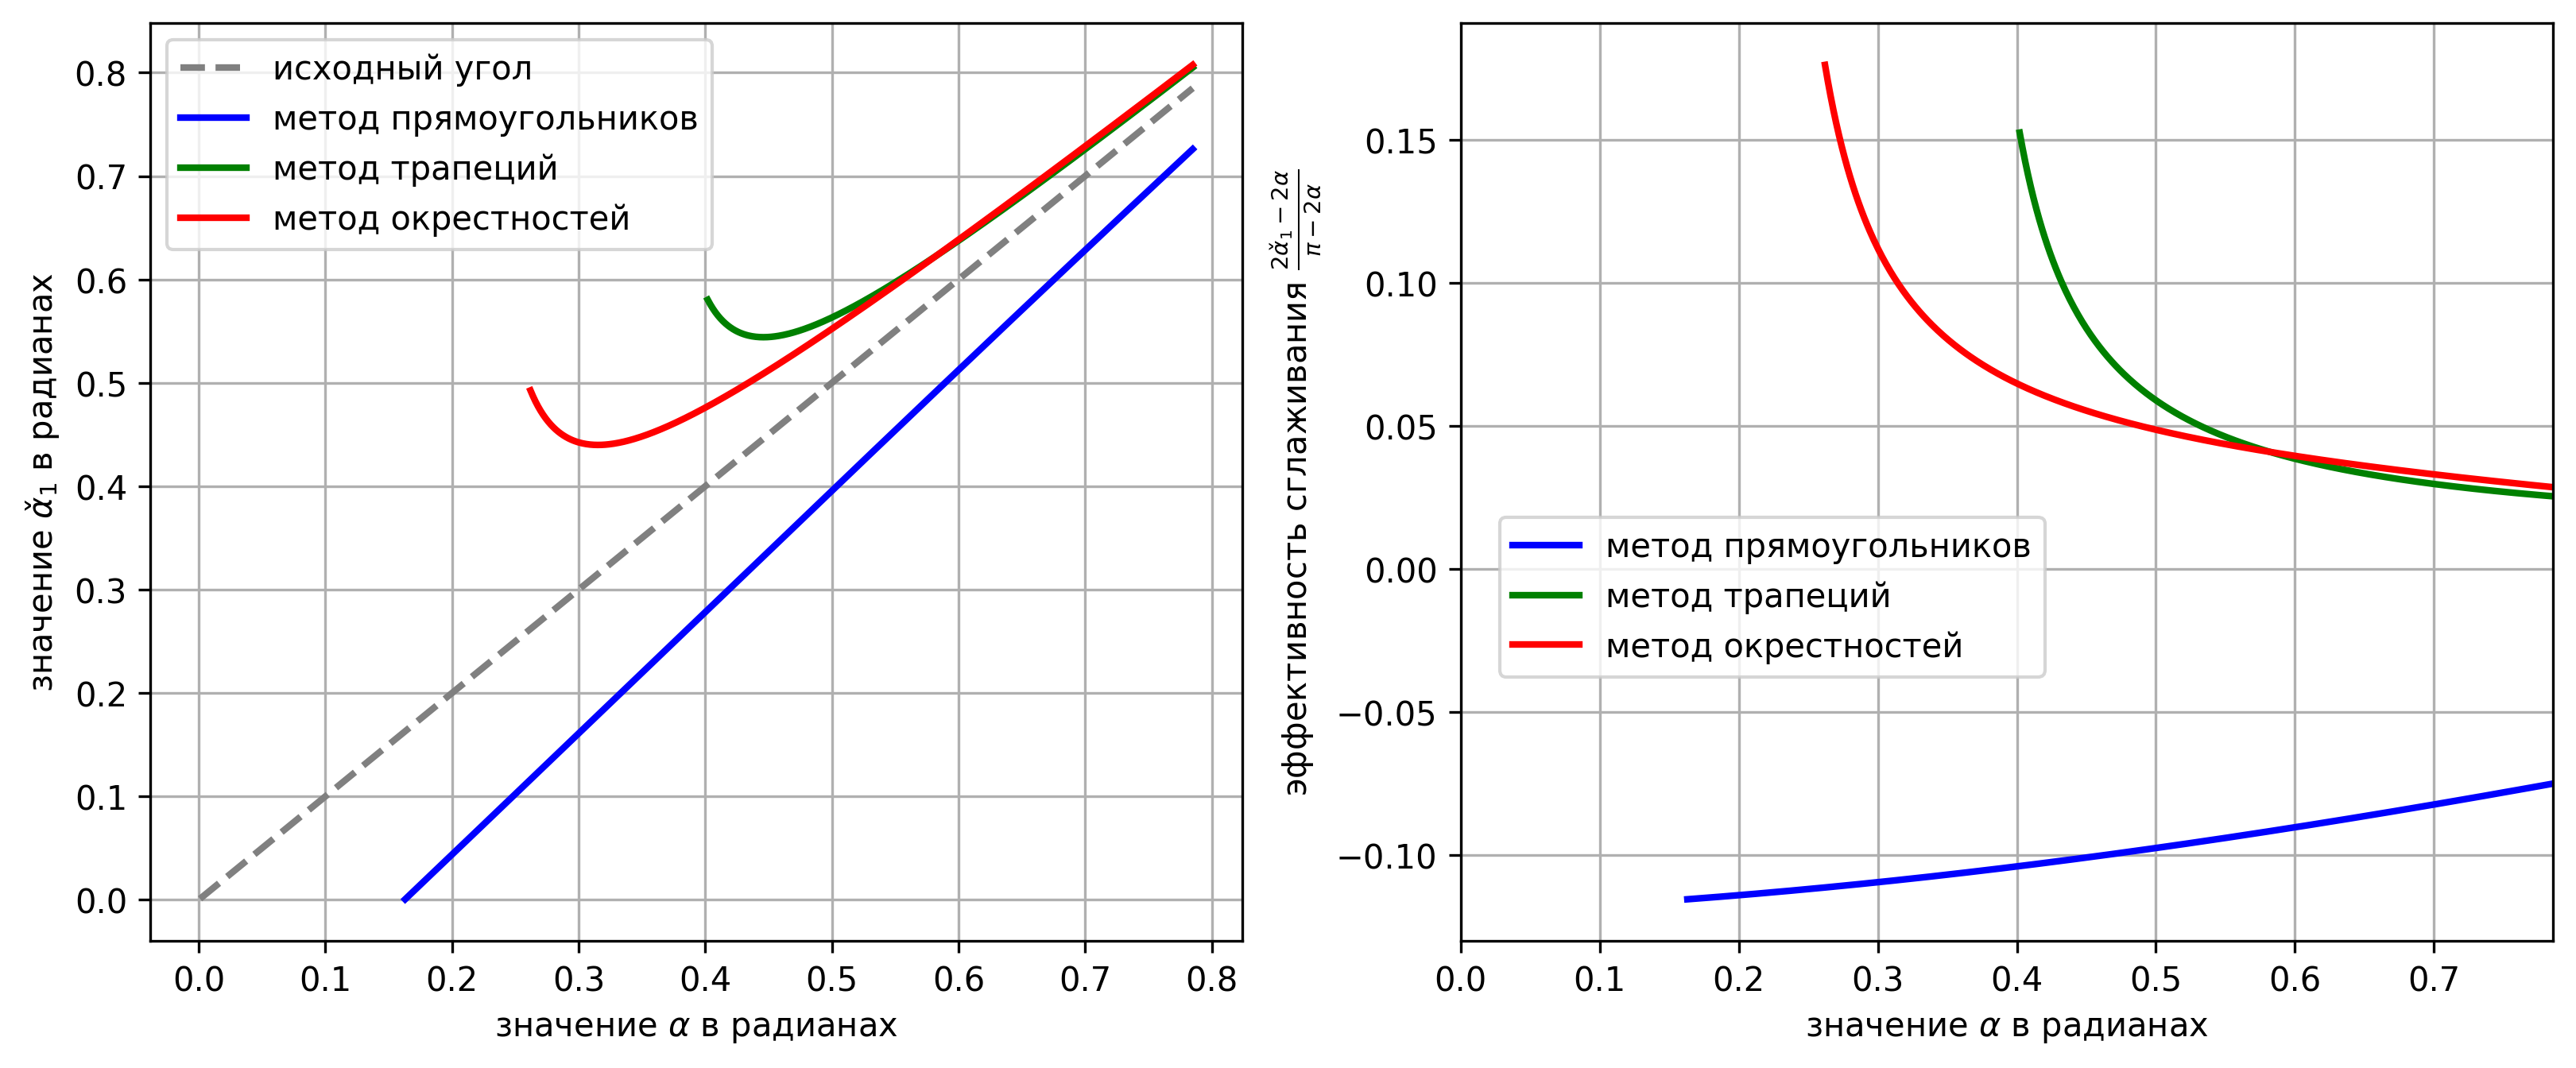
\includegraphics[width=1.0\textwidth]{fig/2dr_cavern_methods_chart.png}
\singlespacing
\captionstyle{center}\caption{Сравнение сглаживания впадины для методов прямоугольников, трапеций и окрестностей.}
\label{fig:text_1_remesh_2d_cavern_methods_chart}
\end{figure}

На основе Леммы~\ref{lem:text_1_cavern_smooth} получим оценки сглаживания угла при впадине при условии постоянного значения $H$ во всех ячейках сетки.

Для метода прямоугольников имеем $h_A = h_B = H$ (см. рис~\ref{fig:text_1_remesh_2d_cavern_methods} слева).

Для метода трапеций необходимо сначала найти высоты двух трапеций $AA'B^{-}B$ и $CC'B^{+}B$ с рис.~\ref{fig:text_1_remesh_2d_cavern_methods} в центре из условия равенства площадей этих трапеций значению $lH$.
Высоты этих трапеций $H^{-}$ и $H^{+}$ получаются из \eqref{eqn:text_1_geo_prim_aa1b1b} с помощью решения квадратного уравнения.
Тогда $h_A = \frac{H^{-}}{\sin \alpha}$, $h_B = \frac{H^{-} + H^{+}}{2 \sin \gamma}$.

В случае метода окрестностей $h_A = \frac{H}{\sin \alpha}$,  $h_B = H$ (см. рис.~\ref{fig:text_1_remesh_2d_cavern_methods} справа).

На рис.~\ref{fig:text_1_remesh_2d_cavern_methods_chart} приведены графики сравнения методов прямоугольников, трапеций и окрестностей в применении к сглаживанию впадин.
При этом используется фиксированная величина смещения ячейки $H = \frac{l}{4}$.
На графике слева показана зависимость изменения сглаженного угла $\check{\alpha}$ от $\alpha$.
На графике справа показана эффективность сглаживания, выраженная формулой $\frac{2 \check{\alpha} - 2 \alpha}{\pi - 2 \alpha}$ (значение 1 означает полное сглаживание пика до угла $\hat{\alpha} = \frac{\pi}{2}$).

Можно отметить, что метод прямоугольников не сглаживает угол, а наоборот, делает его еще более острым (значение эффективности сглаживания меньше нуля).
Метод трапеций показывает лучшую эффективность сглаживания, но с меньшей областью применимости.

Из приведенных оценок на рис.~\ref{fig:text_1_remesh_2d_peak_methods_chart} и рис.~\ref{fig:text_1_remesh_2d_cavern_methods_chart} можно сделать следующие выводы.
С точки зрения сглаживания дефектов сетки метод трапеций неприменим, так как приводит к неконтролируемому росту острых пиков.
Метод прямоугольников неэффективен при сглаживании острых пиков и впадин.
Метод окрестностей позволяет сглаживать как острые пики, так и впадины.

%---------------------------------------------------------------------------------------------------

\subsection{Выводы из главы}

В главе исследовались методы перестроения поверхностной расчетной сетки в двумерном случае.
Рассматривалось перестроение сетки при фиксированных направлениях смещения узлов $N$, совпадающих с их нормалями $\overline{n}_{N}^N$.
Рассматривались известные методы перестроения, основанные на приближении целевой площади ячейки $T$ с помощью геометрических примитивов (методы прямоугольников и трапеций).

Предложен новый метод перестрения поверхностной расчетной сетки -- метод окрестностей -- в котором новое положение узла $N'$ определеятся как точка пересечения $\overline{n}_{N}^N$ с границей окрестности всех инцидентных узлу ячеек.

Выведены аналитические оценки точности методов перестроения расчетной сетки.
Проведен анализ полученных аналитических оценок.
Анализ оценок точности перестроения показал, что наиболее точным методом при малой скорости изменения ледяного покрова является метод трапеций, а точность метода прямоугольников и точность метода окрестностей близки.

Исследована способность рассмотренных методов перестроения сглаживать дефекты расчетной сетки: острые пики и впадины.
Выведены аналитические оценки эффективности сглаживания дефектов расчетной сетки.
Проведен анализ полученных аналитических оценок.
Анализ оценок эффективности сглаживания острых пиков и впадин позволил сделать следующие выводы.
Метод трапеций неприменим для перестроения сетки, так как приводит к неконтролируемому росту острых пиков.
Метод прямоугольников не позволяет сглаживать впадины.
Метод окрестностей наиболее эффективно позволяет сглаживать острые пики, а также позволяет сглаживать впадины.

По результатам проведенных исследований можно заключить, что предложенный метод окрестностей перестроения поверхностной расчетной сетки является наиболее подходящим для моделирования обледенения с точки зрения точности перестроения и сглаживания дефектов сетки.

%---------------------------------------------------------------------------------------------------
